% University of Alberta MSc thesis, built from docs/paper/paper.tex.
% Compile from docs/thesis with: latexmk -pdf thesis.tex
% Class: ualberta (TeX Live, V2.0.0, GPS-compliant title page, roman front matter, PDF/A-3b via the pdfa option).
\documentclass[pdfa,oneside,12pt]{ualberta}

\usepackage[T1]{fontenc}
\usepackage{microtype}
\usepackage{graphicx}
\usepackage{booktabs}
\usepackage{amsmath,amssymb,amsthm}
\usepackage{enumitem}
\usepackage{needspace}
\usepackage{xcolor}
\usepackage{tikz}
\usepackage{adjustbox}
\usepackage{longtable}
\usepackage{capt-of}
% The class defines no thebibliography; natbib only renews it, so declare a placeholder first.
\newenvironment{thebibliography}[1]{}{}
\providecommand\newblock{}
\usepackage[round]{natbib}
\usepackage{xurl}
% The class leaves \thepage undefined until \maketitle; define it so hyperref writes PDF page labels (i, ii, ..., 1, 2, ...).
\providecommand\thepage{\arabic{page}}
\usepackage{hyperref}
\hypersetup{colorlinks, linkcolor={red!50!black}, citecolor={blue!50!black}, urlcolor={blue!80!black}}

% The class uses these table-of-contents lengths without defining them; values from report.cls.
\makeatletter
\providecommand\@pnumwidth{1.55em}
\providecommand\@tocrmarg{2.55em}
\providecommand\@dotsep{4.5}
\makeatother
% The class sets \baselineskip directly, which the next size change undoes; \linespread survives it.
% Values are setspace's for 12pt: 1.25 is one-and-a-half spacing (body, GPS minimum), 1.667 double (abstract).
\renewcommand\onehalfspacing{\linespread{1.25}\selectfont}
\renewcommand\truedoublespacing{\linespread{1.667}\selectfont}

% The paper's figures (recovered with it) come first, so the thesis shows the same figures as the paper.
\graphicspath{{../paper/figs_recovered/}{../paper/figs/}{../../results/llm-test/}}

\theoremstyle{plain}
\newtheorem{theorem}{Theorem}[chapter]
\newtheorem{proposition}[theorem]{Proposition}
\newtheorem{corollary}[theorem]{Corollary}
\newtheorem{lemma}[theorem]{Lemma}
\theoremstyle{definition}
\newtheorem{definition}{Definition}[chapter]
\newtheorem{example}[definition]{Example}
\newcommand{\ess}{\mathrm{ESS}}
\newcommand{\E}{\mathbb{E}}
\newcommand{\R}{\mathbb{R}}
% Result tables were sized for the ICML page; shrink one only if it is wider than the text.
\newcommand{\fittable}[1]{\adjustbox{max width=\textwidth}{\input{#1}}}
% A result table too long for one page: typeset its tabular as a longtable, which breaks across pages.
% longtable steps the table counter itself, so undo that; the caption comes from \captionof.
\newcommand{\longinput}[1]{{\def\theHtable{longtable.\arabic{table}}\let\tabular\longtable\let\endtabular\endlongtable\input{#1}}\addtocounter{table}{-1}}
% Table bodies are single-spaced; the text around them keeps one-and-a-half spacing.
\AtBeginEnvironment{tabular}{\linespread{1}\selectfont}
\AtBeginEnvironment{longtable}{\linespread{1}\selectfont}
% Marks a fact only the author can supply; remove every one before submission.
\newcommand{\todo}[1]{\textcolor{red}{\textbf{[TODO: #1]}}}

% Bibliography: one unnumbered chapter, listed in the table of contents (GPS item 12).
\renewcommand{\bibsection}{\chapter*{\bibname}\addcontentsline{toc}{chapter}{\bibname}}

\title{How Many Demonstrations Is a Task Description Worth? Specificity and Reliability in In-Context Learning}
\author{Trung Quan Nguyen}
\degree{Master of Science}
\specialization{Statistics}
\deptfac{Department of Mathematical and Statistical Sciences}
\convocationdate{2026}

% Plain text only: GPS allows no images or tables, and the class copies it into the PDF/A metadata.
\abstracttext{Task descriptions and demonstrations both convey information about a task, but their relative value is difficult to quantify. We define the predictive effective sample size (ESS) of a description as the number of additional demonstrations required to match its reduction in prediction error. In a Bayesian model of in-context linear regression, we distinguish a description's specificity—the precision of the task information it provides when relevant—from its reliability—the probability that this information applies. Reliable descriptions can replace many demonstrations, with a benefit that depends on task dimension as well as precision. Any fixed positive probability of irrelevance, however, bounds their ESS when no demonstrations are available. Transformers meta-trained on this task approach the Bayesian benchmark and learn how much to trust descriptions from their training distribution. We then test pretrained language models on numerical prediction tasks with explicit probabilistic descriptions and on a semantic classification task. Without reasoning, the models respond weakly to stated precision; with reasoning, several approach the Bayesian reference. With reasoning, they also update a description's reliability from the demonstrations when the prompt states what follows if the description is wrong, but not when it leaves this open. Both behaviors depend on how explicitly the prompt specifies the description's statistical meaning. ESS thus provides a common scale for the information a description offers and the benefit a learner obtains from it.}
\preface{This thesis is an original work by Trung Quan Nguyen, carried out under the supervision of Professor Linglong Kong and Professor Bei Jiang. The author formulated the research questions, designed and carried out the analysis and experiments, and wrote the text; the supervisors provided guidance and feedback throughout.

The thesis is based on the manuscript ``How Many Demonstrations Is a Task Description Worth? Specificity and Reliability in In-Context Learning'' by Bruce Nguyen, the name under which the author writes, prepared in the format of the International Conference on Machine Learning. Chapters~\ref{ch:intro} and~\ref{ch:setup} to~\ref{ch:conclusion} and Appendix~\ref{app:llm-tables} follow that manuscript's text, with its appendices placed in the chapters they support and some added detail; Sections~\ref{sec:outline} and~\ref{sec:future} are new. Chapter~\ref{ch:background} is new, except that it incorporates the manuscript's review of related work, placed in the sections whose topics it concerns. The manuscript has not yet been published.

The research involved no human participants, animals, or personal data, so no research ethics approval was required.

Beyond studying large language models in Chapter~\ref{ch:llm}, the author used tools built on them, Anthropic's Claude Code and OpenAI's Codex, to help write and run experiment code, check derivations, and draft and edit text. The author designed the study, reviewed all code, results, and text, and takes responsibility for them.

The author's salary and the Claude Code and Codex accounts used in this research were paid for by Professor Andrew McGee of the Department of Economics, from funding for his own research.

The author founded Decaude, and this research is part of its research program; the manuscript lists the author's affiliations as Decaude and the University of Alberta.
}
\acknowledgementtext{I am deeply grateful to my family for their unconditional love, which carried me through these years.

I thank my supervisors, Professor Linglong Kong and Professor Bei Jiang, for their guidance and support throughout my program.

I am grateful to Professor Andrew McGee of the Department of Economics for his trust, patience, and generosity.

Finally, I thank God for granting me the strength and wisdom to overcome a life-altering illness during my studies and to complete this work.
}

\begin{document}

\maketitle
\makeabstract\par
\onehalfspacing
\makepreface
% Quotation page (GPS item 4, one page). The author's drawing (front/quote.png, flattened onto white)
% fills the page: its 3160 x 4096 shape matches letter paper, so only a hair is cropped top and bottom.
% The quote sits in the drawing's blank band, about 35-58% of the way down and across the left three
% quarters (measured from the image). The page number stays where it is on every page (GPS); a small
% white patch keeps it legible over the drawing. Needs two runs (remember picture).
\clearpage
\thispagestyle{plain}
\addcontentsline{toc}{chapter}{Quotation}
\begin{tikzpicture}[remember picture, overlay]
\node[inner sep=0] (art) at (current page.center) {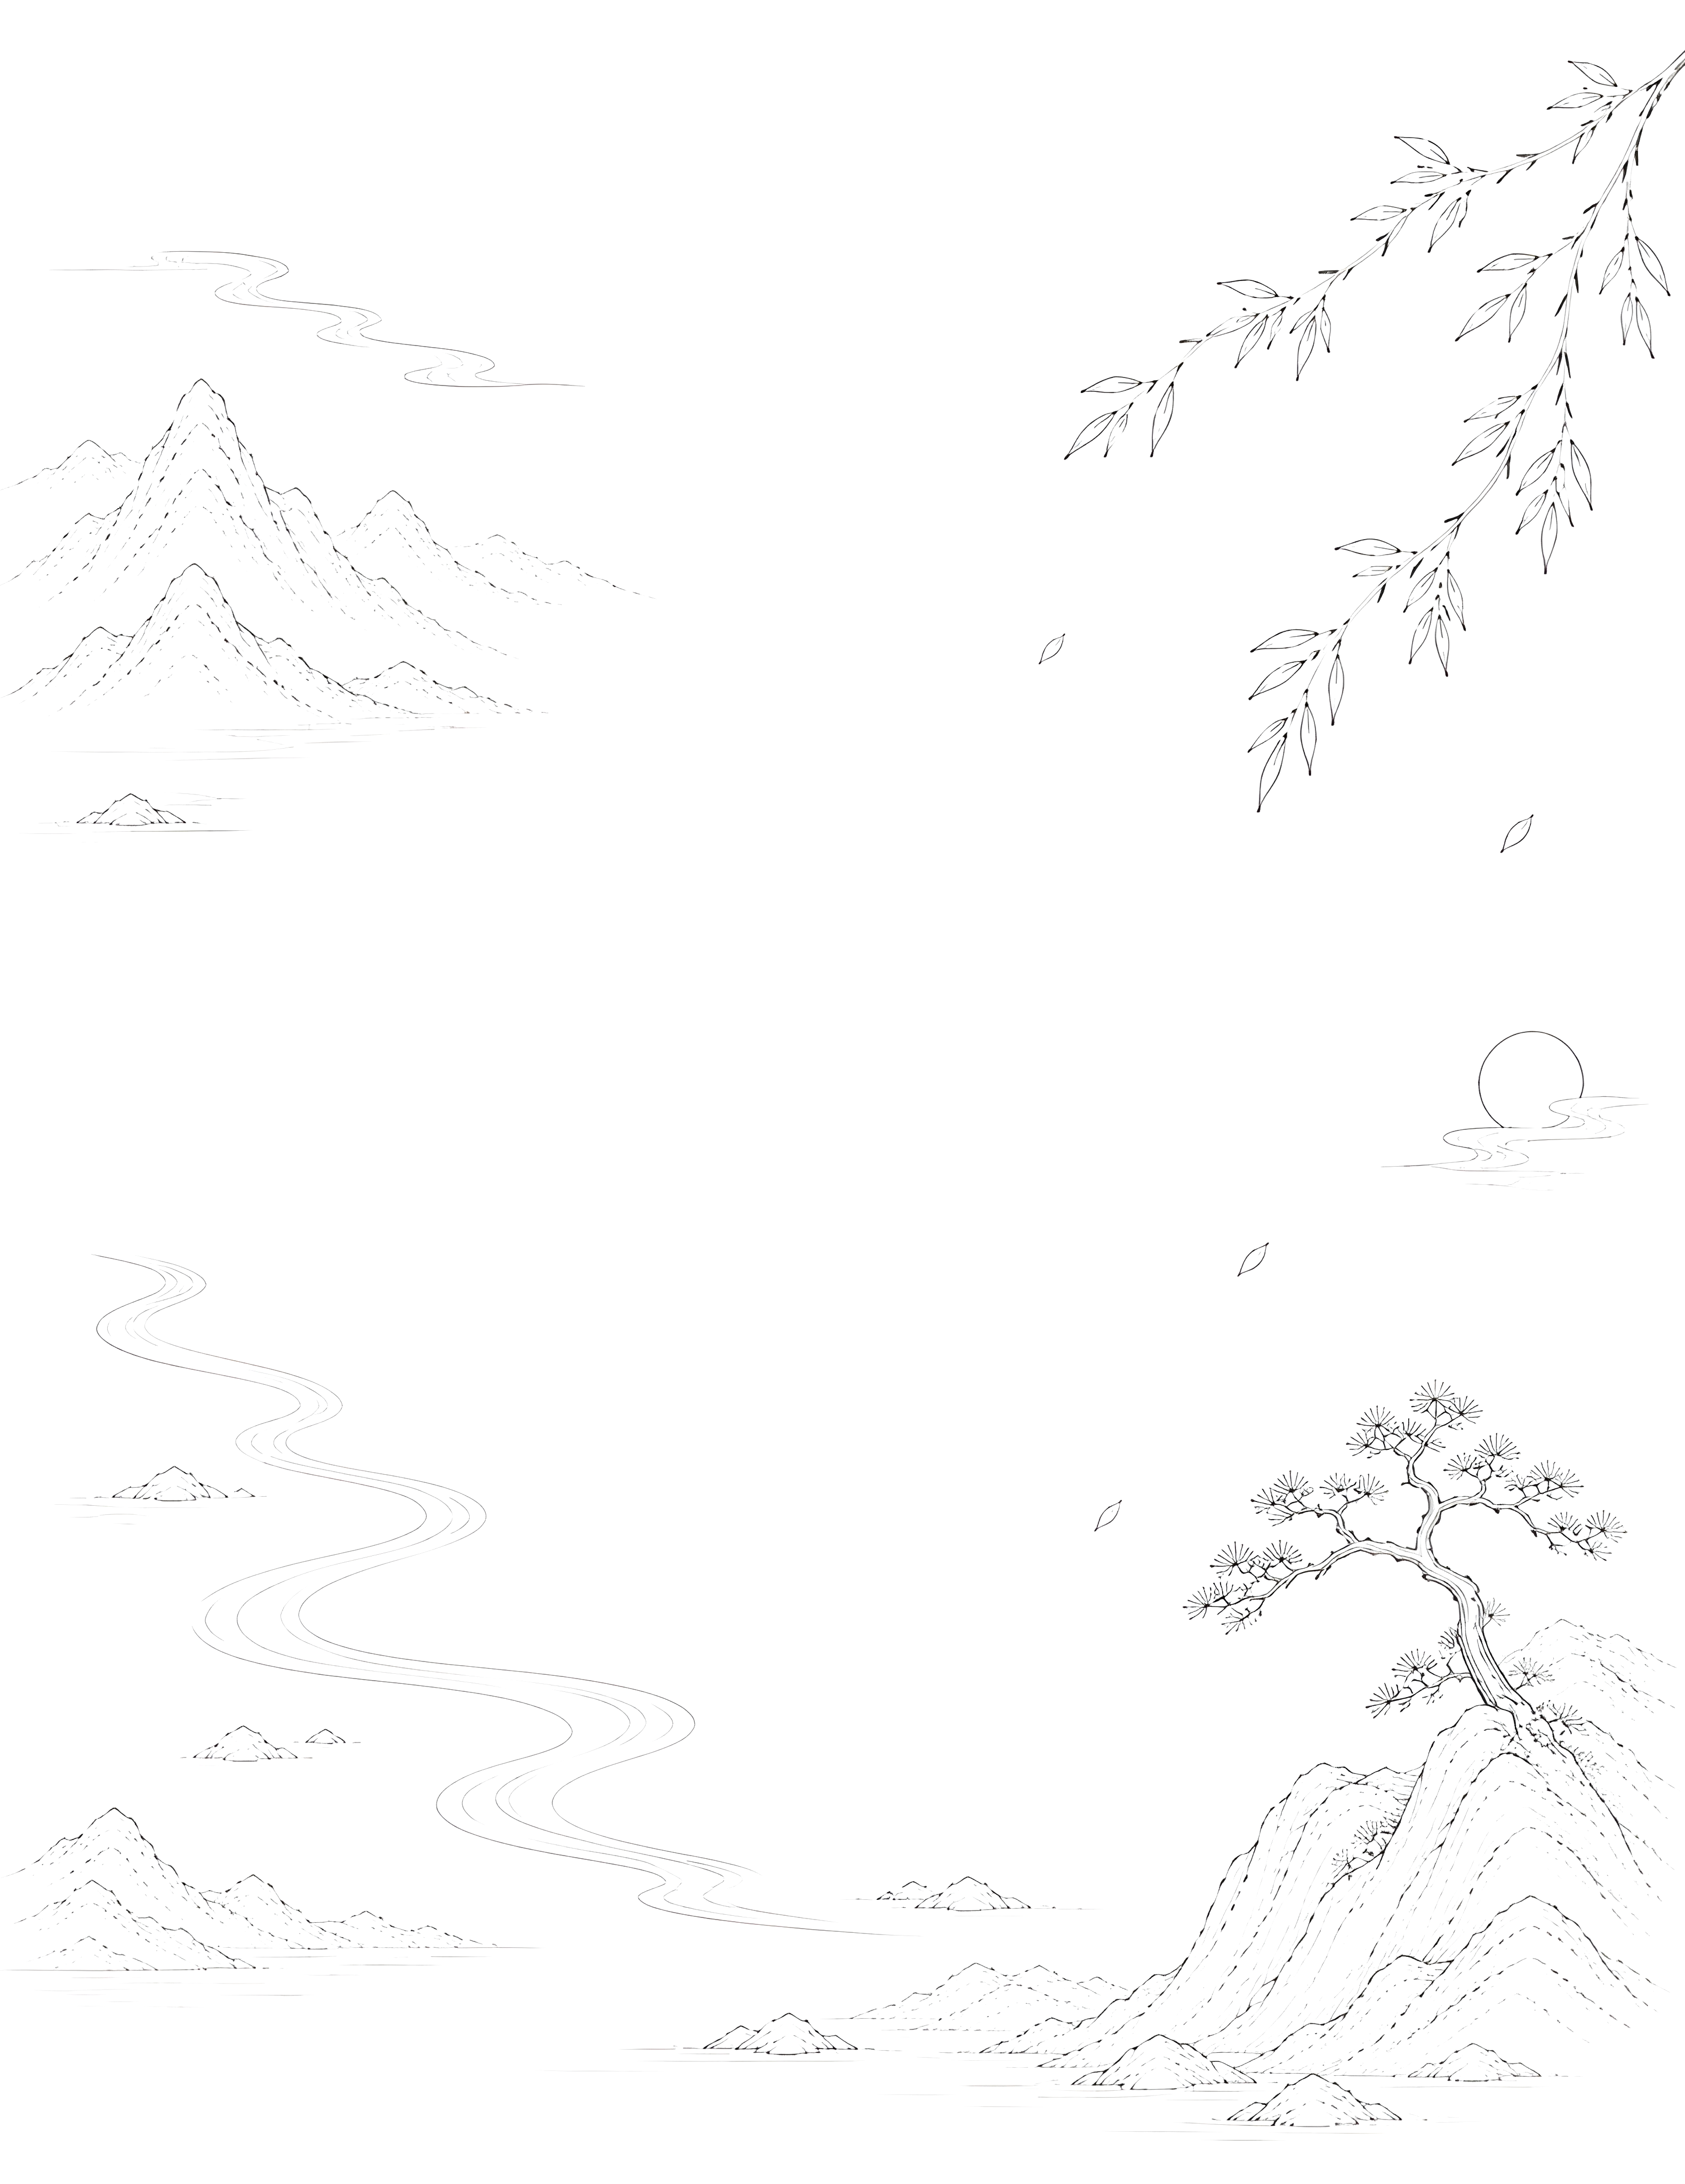
\includegraphics[width=\paperwidth]{front/quote.png}};
\begin{scope}[shift={(art.south west)}, x={(\paperwidth,0)}, y={(0,1.2962\paperwidth)}]
\node[align=center, font=\linespread{1}\selectfont] at (0.42, 0.535) {%
  \textit{The Tao that can be told}\\
  \textit{is not the eternal Tao.}\\
  \textit{The name that can be named}\\
  \textit{is not the eternal name.}\\[8pt]
  {\footnotesize Laozi, \textit{Tao Te Ching}, chapter 1}\\
  {\footnotesize trans.\ Gia-fu Feng and Jane English}};
\end{scope}
% Page-number position measured from the built PDF: centred 288pt from the left, 82pt from the bottom.
\node[fill=white, rounded corners=3pt, minimum width=36pt, minimum height=20pt]
  at ([xshift=288pt, yshift=82pt]current page.south west) {};
\end{tikzpicture}%
\null
\par
\acknowledgements

\tableofcontents
\listoftables
\listoffigures

\bodyoftext
\onehalfspacing

\chapter{Introduction}\label{ch:intro}

\begin{figure}[t]
\centering
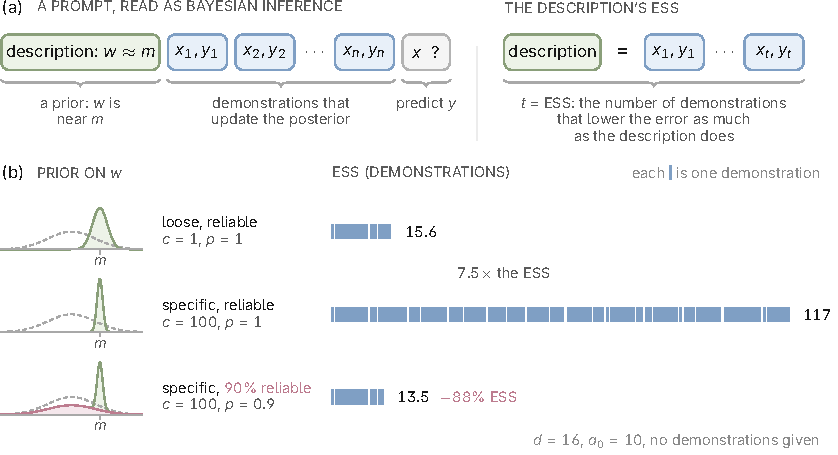
\includegraphics[width=\textwidth]{overview_sq.pdf}
\caption[Measuring a task description in demonstrations]{\textbf{Measuring a task description in demonstrations.} (a) A description provides information about a latent task $w$, and demonstrations supply additional evidence. Its predictive effective sample size (ESS) is the number of additional demonstrations a learner without the description needs to match the error it reaches with the description. The schematic on the right illustrates $n=0$. (b) Description-conditioned task distributions and their Bayes-optimal ESS at $n=0$, $d=16$, and $a_0=10$. Specificity is set by the precision $c$ of the relevant component; reliability $p$ is that component's prior probability. Pink denotes the irrelevant component. Increasing specificity greatly increases ESS when $p=1$, whereas a $10\%$ probability of irrelevance sharply limits this benefit.}
\label{fig:overview}
\end{figure}

Large language models (LLMs) are capable of in-context learning (ICL): given a prompt that specifies a task through a natural-language description, demonstrations, or both, they can predict the output for a new query input \citep{brown2020}. In practice, prompts consist mostly of system instructions, user instructions, skill files, and earlier conversation turns, which typically describe the task rather than demonstrate it \citep{mao2025,patsakis2026}. The balance shifts further as LLMs carry out increasingly long-horizon tasks \citep{kwa2025}, for which demonstrations are costly to provide.

Theories of ICL, however, have mostly focused on prompts consisting of demonstrations alone \citep{xie2022,garg2022,akyurek2023}. The few that include descriptions study only specific types, such as a descriptor that describes the input distribution \citep{huangge2025}, a set of candidate hypotheses \citep{lin2025}, or related datasets supplied as context \citep{zhu2026}; none offers a systematic treatment of descriptions. We therefore ask: how can we characterize natural-language descriptions in general to formally understand and analyze them? And how do descriptions compare, combine, and interact with demonstrations?

We study both questions through the Bayesian view of ICL, in which a model infers a latent task from the demonstrations \citep{xie2022}; a description can then be modeled as a prior over tasks. Descriptions differ in how far they narrow down the task and in whether they apply: ``write this report as an accountant'' leaves most of it open, a step-by-step workflow for each part leaves little, and either may be meant for another task. We formalize these two properties in $d$-dimensional Gaussian linear regression, a standard controlled setting for ICL \citep{garg2022,panwar2024}. Without a description, the coefficients follow a Gaussian baseline prior with variance $a_0$; a description supplies further information about them before demonstrations are observed. A mixture model separates uncertainty about where the task lies from uncertainty about whether the description applies: with probability $p$, the description is relevant, and the coefficients are Gaussian around its center with precision $c$; otherwise, it is independent of the task. We thus characterize a description by two quantities: its \emph{specificity}, set by $c$, and its \emph{reliability}, the prior probability $p$ that it is relevant (Figure~\ref{fig:overview}).

To compare descriptions with demonstrations, we adapt sample-size measures of prior impact and predictive performance \citep{wiesenfarth2020,reimherr2021,lescao2021,selby2025}. For a given learner and prediction loss, a description's \emph{predictive effective sample size} (ESS) at $n$ demonstrations is the additional number of demonstrations needed without the description to reach the same expected error. Standard prior ESS instead matches information, which requires an explicit prior \citep{morita2008}; a network or a language model also brings prior knowledge, acquired in training, but holds it only implicitly in its weights, so only its error can be compared. Computing ESS for both the Bayes-optimal predictor and trained models distinguishes the information available under the statistical model from the benefit realized by a learner.

We then ask how closely trained learners attain the Bayes-optimal ESS. Transformers trained from scratch on the Gaussian model receive each description as an input token and must learn its precision and reliability from their training data. Pretrained language models cannot learn these from the task distribution, so the prompt must state them, as probabilistic statements in numerical mean-estimation tasks. Using a stated precision requires weighting the description and the demonstrations by their precisions, a computation that reasoning may help a model carry out, so we compare models with reasoning enabled and disabled.

% An in-context learner can learn about a task in two ways: a prompt can describe what to do, or it can demonstrate the desired behavior. Most practical prompts combine the two \citep{brown2020}, and task descriptions also appear in system instructions and the files used to configure coding agents \citep{chatlatanagulchai2025}. Yet we lack a common scale for comparing the information supplied by a description with that supplied by examples. When should a precise description replace many demonstrations? When can examples help a learner recognize that a description does not apply?

\section{Main Findings}

Our main findings are as follows:
\begin{itemize}[leftmargin=*,itemsep=2pt,topsep=3pt]
\item \textbf{Precision and dimension determine the value of reliable descriptions.} With fixed positive integer precision $c$, zero-demonstration ESS approaches $c+d+1$ as the baseline prior becomes diffuse (Chapter~\ref{ch:specificity}).
\item \textbf{Uncertain relevance limits zero-demonstration ESS.} Any fixed positive probability of irrelevance imposes a finite ceiling as precision grows. For $d=16$, baseline variance $a_0=10$, and $c=100$, lowering reliability from $1$ to $0.9$ reduces ESS from approximately $117$ to $13.5$. With demonstrations, a learner can also infer whether the description is relevant (Chapter~\ref{ch:reliability}).
\item \textbf{Description use depends on training for Transformers, and on reasoning for language models.} Meta-trained Transformers approach the Bayes-optimal ESS, and their fitted description weight follows the reliability of their training data, even when test descriptions are more reliable. For most pretrained language models tested, enabling reasoning brings their use of stated precision close to the Bayesian reference. When descriptions are in fact unreliable and the prompt says so, GPT-6 Sol with reasoning also matches the reference, which requires inferring relevance from the demonstrations (Chapters~\ref{ch:networks}--\ref{ch:llm}).
\end{itemize}

\section{Outline}\label{sec:outline}

Chapter~\ref{ch:background} reviews in-context learning and its Bayesian interpretation, in-context linear regression and its squared error, the effective sample size of a prior, and robust mixture priors, together with related work. Chapter~\ref{ch:setup} presents the framework: tasks and demonstrations, descriptions as uncertain task information, prediction error, and predictive ESS. Chapter~\ref{ch:specificity} derives the value of a reliable description, with its proofs and the analysis of partial descriptions. Chapter~\ref{ch:reliability} derives the cost of unreliability, with its proofs and the analysis of the Bayesian predictor assuming relevance under misspecification. Chapter~\ref{ch:networks} tests meta-trained Transformers, with their training details and further networks. Chapter~\ref{ch:llm} tests pretrained language models on numerical prediction tasks with explicit probabilistic descriptions, with the evaluation details and further experiments on stated reliability and on a semantic classification task. Chapter~\ref{ch:conclusion} discusses the findings and their limitations, and outlines future work. Appendix~\ref{app:llm-tables} reports the language-model tables at every evaluated demonstration count.

\chapter{Background}\label{ch:background}

In this chapter, we review the ideas that the rest of the thesis builds on. Sections~\ref{sec:bg-icl} to~\ref{sec:bg-linreg} introduce in-context learning, its interpretation as Bayesian inference, and in-context linear regression, a setting in which that interpretation can be computed exactly. Section~\ref{sec:bg-regret} defines the squared error by which we compare learners and gives the error of the Bayesian predictor. Sections~\ref{sec:bg-ess} and~\ref{sec:bg-mixture} present two tools from Bayesian statistics that we later apply to descriptions: the effective sample size of a prior and the robust mixture prior. Finally, Sections~\ref{sec:bg-theory} to~\ref{app:related} review the work most closely related to ours.

\section{In-Context Learning}\label{sec:bg-icl}
A language model takes a sequence of tokens, the prompt, and predicts what comes next. \citet{brown2020} showed that large language models can perform a task specified in the prompt, without any update to their weights. This ability is called in-context learning (ICL). \citet{brown2020} distinguished three kinds of prompts. A zero-shot prompt gives only a natural-language description of the task. One-shot and few-shot prompts add one or several \emph{demonstrations}, solved examples of the task, before the query that the model must answer. We follow their terminology. A demonstration is one input together with its label, and apart from the query we call everything else in the prompt a \emph{description}, whether it is written as a statement about the task or as a command. A prompt can contain both, and our question is how much the description adds to the demonstrations.

How models use the demonstrations is itself an active question. Pretrained models can perform well even when the labels of the demonstrations are replaced by random ones \citep{min2022}, which suggests that they use demonstrations partly to recognize a task they already know. Larger models, however, follow flipped in-context labels more readily \citep{wei2023}. \citet{lin2024} explain both behaviors, retrieving a known task and learning a new one, within a single Bayesian model. A description raises the same question from the other side. Does a model treat it as information about the task, to be weighed against the demonstrations, or does it use it in some other way?

\section{In-Context Learning as Bayesian Inference}\label{sec:bg-bayes}
Theoretical work studies ICL as Bayesian inference over latent tasks \citep{xie2022,panwar2024}, as a learning algorithm implemented in a forward pass \citep{akyurek2023,vonoswald2023}, and as meta-learning across tasks \citep{garg2022,muller2022}. Meta-trained predictors can approximate Bayesian inference under suitable training conditions \citep{genewein2025}, and the learning algorithms that Transformers implement in context approach the Bayes-optimal estimator as the networks grow \citep{akyurek2023}. Agreement can change with training-task diversity or new function classes \citep{raventos2023,panwar2024}, and language-model ICL can violate Bayesian consistency \citep{falck2024}. We adopt the Bayesian view, because it extends naturally from demonstrations to descriptions (Chapter~\ref{ch:setup}).

\citet{xie2022} proposed that ICL can be understood as implicit Bayesian inference. Suppose that pretraining text is generated from latent concepts. A model that predicts such text well must then infer the concept behind each document, and a prompt of demonstrations is evidence about the concept behind the prompt. In this view, a task is a latent parameter $w$, and a prompt contains $n$ demonstrations $D_n=\{(x_i,y_i)\}_{i=1}^n$ and a query $x$. The ideal learner predicts the query's label with the posterior predictive distribution
\begin{equation}\label{eq:bg-predictive}
    f(y \mid x, D_n) = \int f(y \mid x, w)\, f(w \mid D_n)\, dw .
\end{equation}

This view becomes testable when the prior over tasks is known. Consider a Transformer trained on prompts whose tasks are sampled from a known prior. Training on such prompts is called meta-training: the network is trained on many tasks and must infer from the context which task a prompt comes from. The posterior predictive minimizes the expected log loss over the prior (Section~\ref{sec:bg-regret}), and this expected log loss is exactly the training objective. A well-trained network therefore approximates the posterior predictive, whose mean is the Bayes-optimal prediction under squared error (Section~\ref{sec:bg-regret}) \citep{muller2022}. For regression with a Gaussian task prior, meta-trained Transformers behave like the Bayesian predictor, which is ridge regression \citep{akyurek2023, raventos2023, panwar2024}, provided that they are trained on enough distinct tasks \citep{raventos2023}. The Bayesian predictor is then a benchmark against which a network can be measured, and Chapter~\ref{ch:networks} uses it in this way.

\section{In-Context Linear Regression}\label{sec:bg-linreg}
\citet{garg2022} introduced in-context linear regression as a controlled test of ICL. Each prompt has its own task vector $w \sim \mathcal{N}(0, I_d)$, its inputs are drawn as $x_i \sim \mathcal{N}(0, I_d)$, and its labels are $y_i = w^\top x_i$. \citet{garg2022} found that a Transformer trained from scratch on such prompts predicts the query's label about as well as least squares. Later work added label noise, $y_i = w^\top x_i + \epsilon_i$ \citep{akyurek2023, raventos2023}. \citet{raventos2023} also varied the number of distinct tasks seen in training. With few tasks, the network behaves like the Bayesian predictor for a prior over those tasks alone. With enough tasks, it behaves like ridge regression, the Bayesian predictor for the Gaussian prior.

With Gaussian noise and a Gaussian prior, Bayes-optimal prediction has a closed form \citep[Section~14.8]{gelman2013}. We measure labels in units of their noise, so that $y_i \sim \mathcal{N}(w^\top x_i, 1)$. Let the prior be $w \sim \mathcal{N}(m, \Lambda^{-1})$, with center $m$ and precision $\Lambda$. Let $X_n \in \R^{n \times d}$ contain the demonstration inputs as rows, and write $W_n = X_n^\top X_n$. The posterior over $w$ is Gaussian, with covariance and mean
\begin{equation}\label{eq:bg-posterior}
    \Sigma = \big(\Lambda + W_n\big)^{-1}, \qquad \mu = \Sigma \big(\Lambda m + X_n^\top y_{1:n}\big),
\end{equation}
and the posterior predictive for the query is
\begin{equation}\label{eq:bg-gauss-predictive}
    y \mid x, D_n \sim \mathcal{N}\big(\mu^\top x,\; 1 + x^\top \Sigma x\big).
\end{equation}
The predictive variance has two parts. The first, $1$, is the label noise. The second, $x^\top \Sigma x$, is the remaining uncertainty about the task in the direction of the query. Under the baseline prior $\mathcal{N}(0, a_0 I_d)$, the posterior mean $\mu = (W_n + a_0^{-1} I_d)^{-1} X_n^\top y_{1:n}$ is the ridge regression estimate with penalty $a_0^{-1}$. Equation~\eqref{eq:bg-posterior} also shows that a prior acts like additional data. Each demonstration adds $x_i x_i^\top$ to the posterior precision, and the prior adds $\Lambda$. Chapter~\ref{ch:setup} uses this fact to give a description a prior of its own, and in Chapter~\ref{ch:specificity} a reliable description replaces the baseline precision $a_0^{-1}$ with $c$.

\section{Squared Error}\label{sec:bg-regret}
A predictor sees the prompt and gives a number $\hat y$ for the query's label. We score it by squared error. The label is $y = w^\top x + \epsilon$, where the noise $\epsilon$ has mean $0$ and variance $1$ and is independent of the prompt and the task. The expected squared error therefore splits into two parts:
\begin{equation}\label{eq:bg-sq}
    \E\big[(\hat y - y)^2\big] = \E\big[(\hat y - w^\top x)^2\big] + 1 .
\end{equation}
The second part is the noise variance, which is the same for every predictor. Following \citet{garg2022}, we therefore score a predictor by the first part alone, its \emph{prediction error}, or \emph{risk},
\[
    R = \E\big[(\hat y - w^\top x)^2\big],
\]
the expected squared distance from the noiseless label $w^\top x$. A predictor that knows the task predicts $w^\top x$ and has zero error.

Given the prompt, the task is uncertain. For any prediction $\hat y$ computed from the prompt,
\[
    \E\big[(\hat y - w^\top x)^2 \mid x, D_n\big] = \big(\hat y - \E[w^\top x \mid x, D_n]\big)^2 + \operatorname{Var}(w^\top x \mid x, D_n).
\]
The first term vanishes only when $\hat y$ is the posterior mean of $w^\top x$. When tasks are drawn from the prior, the posterior mean therefore has the smallest error of any predictor. We call it the Bayesian predictor and its error Bayes-optimal. It is also the mean of the posterior predictive~\eqref{eq:bg-predictive}. Its error is the expected posterior variance of $w^\top x$. In linear regression, the posterior is Gaussian with covariance $\Sigma$ (Equation~\eqref{eq:bg-posterior}), so the posterior variance of $w^\top x$ is $x^\top \Sigma x$, the part of the predictive variance~\eqref{eq:bg-gauss-predictive} that comes from uncertainty about the task. The query input is independent of the demonstrations, with $\E[x x^\top] = I_d$, so the error of the Bayesian predictor is
\begin{equation}\label{eq:bg-gauss-regret}
    R = \E\big[x^\top \Sigma x\big] = \E \operatorname{tr} \Sigma ,
\end{equation}
the expected trace of the posterior covariance. The error is zero when the posterior has concentrated on the task, and it grows with the uncertainty about the task that remains.

Two standard facts give this trace in the cases that later chapters need. Chapter~\ref{ch:setup} writes $R^{\mathrm{demo}}(n)$ for the error with $n$ demonstrations and no description. With fewer demonstrations than dimensions, $n < d$, the demonstrations say nothing about $d - n$ directions, so under the baseline prior $\mathcal{N}(0, a_0 I_d)$ we have $R^{\mathrm{demo}}(n) \ge (d - n)\,a_0$. Under a flat prior, the limit $a_0 \to \infty$, and with $n \ge d + 2$, the posterior covariance is $W_n^{-1}$, the inverse of a Wishart matrix, and the error is $\E \operatorname{tr} W_n^{-1} = d/(n - d - 1)$ \citep{muirhead1982}. Chapter~\ref{ch:specificity} builds its limits for a reliable description (Proposition~\ref{prop:reliable}) from these two facts.

A predictor that gives a density $g(y \mid x, D_n)$ rather than a number can instead be scored by its log loss, $-\log g(y \mid x, D_n)$. The expected log loss is smallest for the true conditional density of $y$ given the prompt \citep{cover2006}, which is the posterior predictive when tasks are drawn from the prior. Meta-trained networks are often trained with this loss (Section~\ref{sec:bg-bayes}), and so are the networks of Chapter~\ref{ch:networks}. The mean of the posterior predictive is the posterior mean, so a network that minimizes log loss and outputs a predictive mean can be scored by squared error. We use squared error throughout for two reasons. First, it needs only the learner's answer, a number, so it applies to a language model through the number that it writes (Chapter~\ref{ch:llm}). Second, the Bayes-optimal error~\eqref{eq:bg-gauss-regret} has the exact forms above, so the theory in Chapters~\ref{ch:specificity} and~\ref{ch:reliability} can work with exact errors.

Squared error also splits exactly over the components of a mixture. Suppose that a latent indicator $Z$ selects the component that generates the task. By the law of total variance, the posterior variance is the sum of two parts:
\begin{equation}\label{eq:bg-total-variance}
\begin{split}
    \operatorname{Var}(w^\top x \mid x, D_n) ={}& \E\big[\operatorname{Var}(w^\top x \mid x, D_n, Z) \mid x, D_n\big] \\
    &+ \operatorname{Var}\big(\E[w^\top x \mid x, D_n, Z] \mid x, D_n\big).
\end{split}
\end{equation}
The first part is the average variance within the components. The second is the variance of the prediction across the components. Chapter~\ref{ch:reliability} applies this decomposition to a description that may be irrelevant. There, the first part gives the risk of the Bayes-optimal predictor that also observes $Z$, and the second is the excess Bayes risk due to unobserved relevance.

\section{The Effective Sample Size of a Prior}\label{sec:bg-ess}
Bayesian statistics measures the information in a prior by its effective sample size (ESS), the number of observations that would carry the same information. In the conjugate normal model, this number is exact. Suppose that the observations are $y_i \sim \mathcal{N}(w, \sigma^2)$ and the prior is $w \sim \mathcal{N}(m, \sigma^2 / c)$. After $n$ observations with mean $\bar y$, the posterior is
\[
    w \mid y_{1:n} \sim \mathcal{N}\Big(\frac{c\,m + n \bar y}{c + n},\; \frac{\sigma^2}{c + n}\Big).
\]
This is the posterior that $c + n$ observations would give under a flat prior if $c$ of them averaged $m$. The prior is therefore worth $c$ observations, which is its precision measured in units of the precision of one observation. Chapter~\ref{ch:llm} uses this model for its prompt-based Bayesian reference, ignoring negligible boundary effects. The specificity $c$ of a description, defined in Chapter~\ref{ch:setup}, is the same conjugate-prior ESS, counted in each direction in units of direct observations of the task. Chapters~\ref{ch:specificity} and~\ref{ch:reliability} show how the ESS of a description, counted in demonstrations, differs from it.

\paragraph{Prior effective sample size.}
Prior ESS expresses the influence of a prior in observation units, with different definitions matching different statistical quantities \citep{morita2008,neuenschwander2020}. Our comparison is closest to measures based on expected loss \citep{reimherr2021,wiesenfarth2020}. \citet{lescao2021} measure the average horizontal separation of learning curves in prompt-based fine-tuning. \citet{selby2025} compare language-model-elicited priors with data-based predictors by the number of observations needed to match predictive loss. We adapt performance matching to task descriptions at a specified demonstration count, using each learner's own baseline curve, and analyze how precision, dimension, and relevance probability determine predictive ESS.

These definitions extend the ESS beyond the conjugate case in different ways. \citet{morita2008} extend it to any parametric prior. Their ESS is the number of hypothetical observations that, starting from a very vague prior, would give a posterior carrying about the same information as the prior, where information is measured by the curvature of the log density. \citet{neuenschwander2020} require an ESS to be predictively consistent: on average, the ESS of the posterior after $N$ observations should equal the prior's ESS plus $N$. Other definitions let the ESS depend on the current sample, through its size or through the observed data themselves. \citet{reimherr2021} compare a prior with a baseline prior. Their ESS is the number of observations that the baseline would need to perform as well at a given sample size, and it can be negative when the prior and the likelihood conflict. Similarly, the effective current sample size of \citet{wiesenfarth2020} counts the observations that must be added to, or removed from, the current sample for an analysis without the prior to match the analysis with it. Finally, \citet{reznik2026} measures information by predictive log loss to choose the discount of a power prior. A power prior raises the likelihood of historical data, which may not match the current data, to a power between $0$ and $1$.

Our predictive ESS (Definition~\ref{def:ess}) is the number of additional demonstrations that a learner without the description needs to match the learner's error with it. Like the measure of \citet{reznik2026}, it measures information by predictive loss, here squared error.

Our ESS also differs from that of \citet{morita2008} in what it matches. Their ESS matches information. In the conjugate normal model above, a prior of precision $c$ adds $c$ to the posterior precision whatever the number of observations, so it is worth $c$ observations at every sample size. In the same way, a description that raises the prior precision from $a_0^{-1}$ to $c$ in every direction is worth $c - a_0^{-1} = (1-r)\,c$ by their measure, whatever the number of demonstrations in hand. Our ESS matches errors instead. In $d$ dimensions, $n$ demonstrations leave the Bayesian predictor an error of $d/(n - d - 1)$ under a flat prior (Section~\ref{sec:bg-regret}), not the $d/n$ that their expected information would give. Matching errors therefore adds a term that grows with the dimension, the dimension term of Chapter~\ref{ch:specificity}. This term fades as demonstrations accumulate, and with many demonstrations in hand the $\ess_n$ of a reliable description returns to their value (Corollary~\ref{cor:ess}(ii)).

\section{Robust Mixture Priors}\label{sec:bg-mixture}
A prior built from historical data can conflict with the current data. \citet{evans2006} check for such prior--data conflict by asking whether the observed data are surprising under the prior predictive distribution. Clinical trials that borrow historical control data protect against conflict with a robust mixture prior \citep{schmidli2014}. The informative prior $f_I$, derived from the historical data, is mixed with a vague prior $f_V$:
\[
    f(w) = p\, f_I(w) + (1 - p)\, f_V(w).
\]
The posterior is then a mixture of the two component posteriors, and the weight on the informative component is updated in proportion to $p$ times its marginal likelihood. When the data agree with the informative component, its weight grows, and the trial borrows the historical information. When they conflict, the weight moves to the vague component, and the analysis falls back on the current data.

A description is a prior of the same kind. It may describe the task at hand, but it may also have been written for another task, or it may simply be wrong. Chapter~\ref{ch:setup} therefore models a description as a robust mixture prior whose weight is its reliability $p$, the probability that the description is relevant. Chapter~\ref{ch:reliability} calls the updated weight the posterior relevance probability $\pi_n$ and shows how reliability affects the description's ESS.

\section{Descriptions in Theories of ICL}\label{sec:bg-theory}
Additional task information has been studied through input-distribution descriptions \citep{huangge2025}, candidate hypotheses \citep{lin2025}, task-group mixtures \citep{lin2024}, changing instruction influence \citep{tong2026}, and related datasets supplied as context \citep{zhu2026}. We use explicit Bayesian predictors to quantify how such information changes the demonstrations needed for a given prediction error.

In some of these theories, the description is a set of tokens that indicate a hypothesis class \citep{lin2025} or carry the mean of the inputs \citep{huangge2025}. These theories generally do not measure the value of a description in demonstrations, and they do not model the possibility that it is irrelevant. For example, \citet{huangge2025} show that a learner can use the description token to predict better, but they do not say how many demonstrations it is worth or what it is worth when it may be wrong. The Bayesian theory of \citet{xie2022} models the prompt as demonstrations alone. We keep its view of the prompt as evidence about a latent task and add a description, which induces a distribution over tasks before the demonstrations are observed. Our networks in Chapter~\ref{ch:networks} use the prefix embedding of \citet{huangge2025}, in which the description is a single token placed before the demonstrations. The work closest to our setting is that of \citet{zhu2026}, who show that a Transformer given a prefix of related datasets performs amortized hierarchical Bayesian prediction. We measure the value of such conditioning information in demonstrations, and we allow it to be irrelevant.

\section{Descriptions and Priors in Pretrained Language Models}\label{sec:bg-llm}

Task summaries distilled from demonstrations can replace the examples in context \citep{honda2025}. Other studies report weak sensitivity to instruction relevance \citep{webson2022} or limited benefits from repository instruction files \citep{gloaguen2026}. \citet{gupta2025} compare explicitly stated coin biases with observations and evaluate the predictions against Bayesian references. Concurrent work studies how reasoning and code execution affect language models' approximation of Bayesian posteriors \citep{filbry2026}. Our numerical experiments vary stated precision and reliability separately, with controls that hold the description center and demonstrations fixed. Code execution is disabled in the main runs. Section~\ref{app:related} discusses further connections.

\section{Additional Related Work}\label{app:related}

\paragraph{Task descriptions and demonstrations.}
\citet{weller2020} formalize learning from task descriptions by distinguishing the latent task, its natural-language description, and individual input--output examples. We use \emph{task description} for information about the task supplied in the prompt, including a numeric description token in the meta-trained setting and probabilistic statements or policy constraints in the language-model experiments. A \emph{demonstration} is an observed input--output example; in scalar mean estimation, it is an observation at the fixed input $x=1$. Summaries distilled from demonstrations can serve as descriptions \citep{honda2025}; our controlled experiments instead specify the joint distribution of task, description, and demonstrations.

\paragraph{Prior information and uncertain relevance.}
The two-component construction is related to robust mixture priors, which combine informative and baseline distributions and update their component weights after observing data \citep{schmidli2014}. Our mixture is specified directly, rather than derived from a historical-data meta-analysis. Reliability $p$ is the prior probability of the description-conditioned component; $\pi_n$ is its posterior probability. Averaging component predictions using $\pi_n$ is Bayesian model averaging \citep{hoeting1999}. The experimental comparison that retains $p$ instead averages with prior weights. Fixed prior weights in a robust prior still yield updated posterior weights.

Our relevance terminology also has a conceptual precedent in information fusion, where relevance is distinguished from truthfulness \citep{pichon2012}. That work uses belief functions; our probability model is different. In our model, an irrelevant description is independent of the task and may happen to agree with it. Thus irrelevance is a generating condition, whereas prior--data conflict concerns disagreement between prior information and observed data. Related approaches discount external information according to predictive loss \citep{reznik2026} or accommodate conflict with heavy-tailed distributions \citep{ohagan2012}.

\paragraph{Specificity and description weights.}
Specificity takes a concrete form in each setting. In the isotropic Gaussian model, it is represented by prior precision $c$; a partial description also specifies the number $k$ of constrained directions. In the semantic experiment, broad and specific notes leave different numbers of compatible policies. These constructions do not define a common numerical scale across tasks. In Gaussian mean estimation, the reference combines the prior mean and sample mean with weights proportional to their precisions \citep{neuenschwander2020}. Fitted and per-response description weights summarize model predictions. Their normalized values can be compared with posterior component probabilities, but need not themselves be probabilities.

\paragraph{Effective sample size and predictive comparisons.}
Prior ESS has several definitions, including matching local information \citep{morita2008}, matching expected posterior loss \citep{reimherr2021}, and quantifying sample savings at a target estimation accuracy \citep{wiesenfarth2020}. Our definition follows the risk-matching approach but evaluates population prediction error and allows a non-Bayesian learner. Its dependence on the demonstration count is part of the definition. The word \emph{predictive} specifies what is matched; it does not assert the additive predictive-consistency property studied by \citet{neuenschwander2020}.

Two predictive comparisons are especially close. \citet{lescao2021} average horizontal data advantages over an accuracy range in supervised fine-tuning; we evaluate a pointwise difference in demonstration counts. \citet{selby2025} compare priors elicited from language models with data-based predictors by the observations needed to match predictive loss; we study descriptions supplied to a learner and how their benefit changes after demonstrations. Beyond ICL, an instruction can replace up to $100$ execution examples in the fine-tuning settings studied by \citet{cook2026}. \citet{wenliang2026} compare optimized prompts with demonstrations in terms of their length and effect. They treat a prompt as conditioning for a Bayesian sequence predictor and find that an optimized prompt can be shorter than demonstrations with the same effect.

\paragraph{Demonstrations, text, and probabilistic prediction.}
Other work examines semantic priors and flipped labels \citep{wei2023}, weak dependence on demonstration labels \citep{min2022}, Bayesian scaling laws \citep{arora2025}, and Bayesian reference curves for in-context function learning \citep{akata2026}. Text supplied alongside numbers can change numerical predictions \citep{requeima2024}, and models estimate a density from numbers in context like a kernel density estimator with an adaptive bandwidth \citep{liu2025}. Related work studies how language-model outputs compare with Bayesian inference and how training can improve probabilistic reasoning \citep{qiu2026}; \citet{he2025} examine Bayesian consistency during iterative reasoning on open-ended questions. Our numerical experiments state uncertainty explicitly, allowing comparison with a specified Bayesian reference as precision and relevance probability vary. The semantic task extends this comparison to ordinary-language constraints on a finite family of classification policies.

In the reference comparisons, the learning curves of pretrained models approach a Bayesian reference on synthetic tasks with a known optimum \citep{akata2026}, and \citet{arora2025} model in-context learning curves with a Bayesian scaling law that includes a task prior. Where \citet{min2022} and \citet{wei2023} vary the labels of the demonstrations, we ask the converse question: does a model weigh a description according to what the prompt says about it?

\chapter{Framework}\label{ch:setup}

\paragraph{Tasks and demonstrations.}
We use the standard noisy in-context linear regression setting \citep{garg2022,raventos2023}. A task is a vector $w\in\R^d$ drawn from the baseline prior $\mathcal{N}(0,a_0 I_d)$. A prompt contains $n$ demonstrations $D_n=\{(x_i,y_i)\}_{i=1}^n$ and a query $x$, where
\[
x_i,x\overset{\mathrm{iid}}{\sim}\mathcal{N}(0,I_d),\qquad
y_i=w^\top x_i+\epsilon_i,\quad
\epsilon_i\overset{\mathrm{iid}}{\sim}\mathcal{N}(0,1).
\]
The parameter $a_0>0$ controls variation across tasks. Numerical illustrations in Chapters~\ref{ch:specificity}--\ref{ch:reliability} use $d=16$ and $a_0=10$.

\paragraph{Descriptions as uncertain task information.}
A description supplies a center $m\in\R^d$. Its \emph{specificity} is a precision $c\geq 1/a_0$, and its \emph{reliability} is a probability $p\in[0,1]$. Write $r=(ca_0)^{-1}\in(0,1]$ for the fraction of baseline variance remaining when the description is relevant. With an unobserved relevance indicator $Z\sim\mathrm{Bernoulli}(p)$, independent of $m$, we generate
\begin{align*}
m&\sim\mathcal{N}(0,(1-r)a_0I_d),\\
w\mid m,Z=1&\sim\mathcal{N}(m,ra_0I_d),\\
w\mid m,Z=0&\sim\mathcal{N}(0,a_0I_d).
\end{align*}
Thus the description induces the mixture prior
\[
w\mid m\sim p\,\mathcal{N}(m,c^{-1}I_d)
 +(1-p)\,\mathcal{N}(0,a_0I_d),
\]
as in robust mixture priors for potentially incompatible information \citep{schmidli2014}. Both relevance branches have the same marginal task distribution, $w\sim\mathcal{N}(0,a_0I_d)$. Consequently, the comparison with and without a description does not change the task population.

A description is \emph{reliable} when $p=1$ and \emph{unreliable} when $p<1$. Greater $c$ means greater specificity conditional on relevance. The model separates uncertainty within the described region from uncertainty about whether that region applies. It does not assume that every natural-language description can be summarized by these two scalars.

A relevant description splits the baseline variance $a_0$ into the part $(1-r)a_0$ that $m$ resolves and the part $ra_0$ that it leaves. Because the observation noise has unit variance, $c$ is measured in demonstrations: in each direction, it is the ESS that \citet{morita2008} assign to a normal prior. We call a description \emph{loose} when $c$ is small relative to $d$ and \emph{specific} when $c$ exceeds $d$. At $d=16$ and $a_0=10$, a description with $c=1$ ($r=0.1$) is loose, and one with $c=100$ ($r=0.001$) is specific.

\paragraph{Prediction error.}
For a prediction $\hat y$ of the query response, we measure error against its conditional mean:
\begin{equation}\label{eq:regret}
R=\E\big[(\hat y-w^\top x)^2\big].
\end{equation}
This excludes irreducible query noise. The expectation is over tasks, descriptions, demonstrations, and queries. For a fixed learner, let $R^{\mathrm{desc}}(n)$ and $R^{\mathrm{demo}}(n)$ denote its errors with and without a description. We write $R^{\mathrm{desc}}_{p=1}(n)$ for the reliable case.

\begin{definition}[Predictive effective sample size]\label{def:ess}
Given $n$ demonstrations, let $n^*$ be the smallest $t\geq0$ such that $R^{\mathrm{demo}}(t)=R^{\mathrm{desc}}(n)$. When this crossing exists, the ESS of the description is
\[
\ess_n=n^*-n.
\]
We interpolate $R^{\mathrm{demo}}$ between available demonstration counts: linearly in $t$ for the theory and meta-trained models, and in $\log t$ for language models. For measured curves, we use the first crossing within the observed range and report out-of-range values as bounds. The language-model conventions are detailed in Section~\ref{app:llm}. If $R^{\mathrm{desc}}(n)>R^{\mathrm{demo}}(t)$ for all $t\geq0$, we report $\ess_n\leq-n$.
\end{definition}

ESS measures a horizontal displacement of a learning curve: $\ess_n=10$ means that $n$ demonstrations plus the description match the error of $n+10$ demonstrations without it. For a decreasing baseline curve, a negative value indicates increased error at the same demonstration count. Each model is evaluated against its own curve, so ESS measures the description's value \emph{to that learner}; a large ESS alone does not imply low absolute error. Under the correctly specified Bayesian model, descriptions cannot increase expected risk, and ESS is nonnegative.

Because $R$ averages over descriptions, the ESS belongs to a kind of description, determined by $c$ and $p$, rather than to a particular value of $m$.

\chapter{The Value of a Reliable Description}\label{ch:specificity}

For $p=1$, the Bayesian predictor uses the posterior mean of $w^\top x$. Its risk is the expected trace of the posterior covariance of $w$. Let $X_n$ contain the demonstration inputs as rows and write $W_n=X_n^\top X_n$. Then
\begin{align*}
R^{\mathrm{demo}}(n)&=\E\operatorname{tr}(a_0^{-1}I_d+W_n)^{-1},\\
R^{\mathrm{desc}}_{p=1}(n)&=\E\operatorname{tr}(cI_d+W_n)^{-1}.
\end{align*}
The description replaces baseline precision $a_0^{-1}$ with $c$. Its predictive value is not, however, determined by this precision difference alone.

\begin{proposition}[Reliable descriptions]\label{prop:reliable}
Let $p=1$.
\begin{enumerate}[label=(\roman*),nosep,leftmargin=*]
\item With $r\in(0,1]$ fixed, $\ess_0\geq(1-r)d$, and $\ess_0\to(1-r)d$ as $a_0\to\infty$.
\item With positive integer $c$ fixed, $\ess_0\to c+d+1$ as $a_0\to\infty$.
\end{enumerate}
\end{proposition}

The two limits describe different regimes (proof in Section~\ref{app:specificity}). In the first, the description removes a fixed fraction of uncertainty in every direction. Each of the first $d$ demonstrations constrains one direction, so reducing variance across all directions can save approximately $(1-r)d$ demonstrations. In the second, the description retains a fixed absolute precision while the baseline prior becomes diffuse. Without a description, the limiting risk is $d/(n-d-1)$ for $n>d+1$ \citep{muirhead1982}; the description alone has risk $d/c$. These risks match at $n=c+d+1$. The integer restriction makes the crossing coincide with a measured count under linear interpolation.

This $d+1$ contribution reflects the cost of learning a $d$-dimensional task from random inputs. Matching average information would count only the added precision $c-a_0^{-1}$; matching predictive error also accounts for the random design. We refer to the additional contribution as the \emph{dimension term}. It is substantial when $c$ is small relative to $d$, whereas precision dominates when $c$ is large. This interpretation concerns the stated limits, rather than an exact additive formula for every finite $a_0$ and $n$.

The comparison with matching information can be made explicit in this limit. For a normal prior, the ESS of \citet{morita2008} is the ratio of the observation variance to the prior variance, so raising the baseline precision $a_0^{-1}$ to $c$ is worth $c-a_0^{-1}=(1-r)c$ demonstrations under their definition, at every $n$. With a diffuse baseline prior, $n$ demonstrations leave risk $d/(n-d-1)$, not the risk $d/n$ that their expected information would suggest. Setting $d/n$ equal to the description's risk $d/c$ gives $n=c$; setting $d/(n-d-1)$ equal to it gives $n=c+d+1$. The dimension term is the gap between the two.

\begin{figure}[t]
\centering
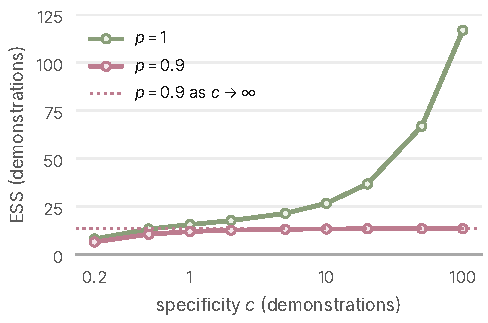
\includegraphics[width=0.75\textwidth]{ess_sq.pdf}
\caption[Reliability limits the benefit of greater specificity without demonstrations]{\textbf{Reliability limits the benefit of greater specificity without demonstrations.} Bayesian $\ess_0$ versus specificity $c$, for $p=1$ and $p=0.9$, at $d=16$ and $a_0=10$. The dotted line is the finite ceiling for $p=0.9$ as $c\to\infty$. Estimates use eight batches of $4{,}000$ prompts; standard errors are below $0.02$ demonstrations.}
\label{fig:ess}
\end{figure}

At $d=16$ and $a_0=10$, a reliable description with $c=1$ has ESS $15.6$, compared with the lower bound $(1-r)d=14.4$. Increasing $c$ to $100$ raises ESS to approximately $117$ (Figure~\ref{fig:ess}). As demonstrations accumulate, the dimension benefit disappears: $\ess_n\to c-a_0^{-1}$ (Corollary~\ref{cor:ess}). For example, after $100$ demonstrations the $c=1$ description is worth $1.1$ demonstrations, close to its added precision of $0.9$.

\paragraph{Coverage matters as well as precision.}
A description may constrain only $k<d$ directions. For any fixed precision $c>0$, its zero-demonstration ESS approaches $k$ as $a_0\to\infty$; increasing that fixed precision does not remove uncertainty in the other directions. With many demonstrations, its ESS instead approaches $k(c-a_0^{-1})/d$ (Proposition~\ref{prop:partial}). A precise partial description can therefore become more valuable as demonstrations resolve what it leaves unspecified. At $d=16$, $k=8$, and $c=100$, ESS increases from $8.1$ without demonstrations to $36$ with $100$ demonstrations (Table~\ref{tab:partial}).

\begin{table}[t]
\centering\small
\setlength{\tabcolsep}{3pt}
\caption[Demonstrations can increase the value of a precise partial description]{\textbf{Demonstrations can increase the value of a precise partial description.} Bayes-optimal ESS for a reliable description of $k$ of $d=16$ directions, with $a_0=10$. The case $k=16$ is a complete description. Each block reports ESS after $n$ demonstrations and its large-sample limit $(1-r)ck/d$. Estimates use eight batches of $2{,}000$ prompts; standard errors are at most $0.23$.}
\label{tab:partial}
\vspace{3pt}
\fittable{../paper/figs/partial_table.tex}
\end{table}

\section{Reliable Descriptions}\label{app:specificity}

\paragraph{Notation and risk.}
Write $\varepsilon = 1/a_0$, let $X_n\in\R^{n\times d}$ contain the demonstration inputs as rows, and set $W_n=X_n^\top X_n$. For $\kappa>0$, define
\[
R^{\kappa}(n)=\E\operatorname{tr}(\kappa I_d+W_n)^{-1}.
\]
Thus $R^{\mathrm{demo}}=R^{\varepsilon}$ and $R^{\mathrm{desc}}_{p=1}=R^c$. These identities follow from the posterior covariance under Gaussian linear regression. Conditional on the prompt, the posterior mean minimizes squared prediction error, and the independent query satisfies $\E[xx^\top]=I_d$. Averaging its conditional error $x^\top\Sigma x$ therefore gives $\E\operatorname{tr}\Sigma$.

Throughout the proofs, $d$ is a positive integer, $a_0>0$, $c\ge\varepsilon$, $r=1/(ca_0)\in(0,1]$, and $p\in[0,1]$. Noninteger sample sizes refer to linear interpolation between the risks at adjacent integers.

\paragraph{Wishart identities.}
We use three standard properties of $W_n$.
\begin{enumerate}[label=(W\arabic*),leftmargin=*]
    \item If $n<d$, then $W_n$ has rank $n$ almost surely. Consequently, $(\kappa I_d+W_n)^{-1}$ has $d-n$ eigenvalues equal to $1/\kappa$.
    \item If $n\ge d$ and $e$ is a fixed unit vector, then $(e^\top W_n^{-1}e)^{-1}\sim\chi^2_{n-d+1}$ \citep[Theorem~3.2.12]{muirhead1982}. Hence
    \[
    \E\operatorname{tr}W_n^{-1}=\frac{d}{n-d-1}\quad(n\ge d+2),
    \]
    whereas this expectation is infinite for $n=d$ and $n=d+1$.
    \item For fixed $d$, as $n\to\infty$,
    \[
    \E\operatorname{tr}W_n^{-2}=\frac{d}{n^2}+O(n^{-3}),
    \qquad
    \E\operatorname{tr}W_n^{-3}=O(n^{-3})
    \]
    \citep{vonrosen1988}.
\end{enumerate}
The Sherman--Morrison identity implies that an additional demonstration strictly decreases the expected trace of the posterior covariance. Thus $R^\kappa(n)$ is strictly decreasing, and (W2) implies that it tends to zero. Its linear interpolation is therefore continuous and strictly decreasing. In the correctly specified joint model, conditioning on the description cannot increase expected posterior variance, so $R^{\mathrm{desc}}(n)\le R^{\mathrm{demo}}(n)$ and the Bayes-optimal ESS is nonnegative.

\begin{proof}[Proof of Proposition~\ref{prop:reliable}]
A reliable description without demonstrations has risk
\[
R^{\mathrm{desc}}_{p=1}(0)=\frac{d}{c}=ra_0d.
\]

\emph{(i) Fixed variance reduction.}
By (W1), $R^\varepsilon(n)\ge(d-n)a_0$ for $n<d$; the inequality also holds trivially for $n\ge d$. Linear interpolation preserves this bound, so
\[
R^{\mathrm{demo}}(t)\ge(d-t)a_0\qquad(t\ge0).
\]
For $t<(1-r)d$, the right-hand side exceeds $ra_0d$. The matching sample size must therefore satisfy $\ess_0\ge(1-r)d$.

For every integer $n$,
\[
\frac{R^\varepsilon(n)}{a_0}
=\E\operatorname{tr}(I_d+a_0W_n)^{-1}
\longrightarrow(d-n)^+
\qquad\text{as }a_0\to\infty.
\]
Indeed, an eigenvalue $1/(1+a_0\lambda)$ is bounded by one and converges to the indicator of $\lambda=0$, so dominated convergence and the almost-sure rank of $W_n$ apply. The same limit holds at every real $t$ by interpolation. For fixed $r\in(0,1)$, the limiting curve crosses $rd$ at the unique point $t=(1-r)d$. Strict monotonicity then gives convergence of the crossing. For $r=1$, the description is uninformative and $\ess_0=0$ for every $a_0$, giving the same conclusion.

\emph{(ii) Fixed precision.}
For fixed $c>0$, the description risk $d/c$ is independent of $a_0$. As $a_0\to\infty$, monotone convergence, (W1), and (W2) give
\[
R^\varepsilon(n)\longrightarrow
\begin{cases}
+\infty,&n\le d+1,\\[2pt]
\displaystyle\frac{d}{n-d-1},&n\ge d+2.
\end{cases}
\]
If $c$ is a positive integer, the finite part of this limiting curve equals $d/c$ at the integer $n=c+d+1$. For every fixed point below this crossing the limiting risk is larger than $d/c$, and for every fixed point above it the limiting risk is smaller. The crossing of the interpolated finite-$a_0$ risk therefore converges to $c+d+1$. The integer condition ensures that the equality occurs at a grid point; linear interpolation does not in general preserve the same expression for noninteger $c$.
\end{proof}

\paragraph{Large-sample expansion.}
For fixed $d$ and $\kappa$, commuting $W_n$ with $\kappa I_d$ gives
\[
(\kappa I_d+W_n)^{-1}
=W_n^{-1}-\kappa W_n^{-2}
+\kappa^2W_n^{-2}(\kappa I_d+W_n)^{-1}.
\]
The final term is positive semidefinite and bounded above by $\kappa^2W_n^{-3}$. Using (W2) and (W3),
\begin{equation}\label{eq:extra}
R^\kappa(n)=\frac{d}{n-d-1}-\frac{\kappa d}{n^2}+O(n^{-3}).
\end{equation}
An additional demonstration reduces the leading term by $d/n^2+O(n^{-3})$. Thus a fixed change in prior precision and a fixed change in sample size affect risk at the same order. This observation underlies the large-$n$ ESS limits below.

\section{Partial Descriptions}\label{app:partial}

A reliable description may constrain only part of a task. Suppose it leaves a fraction $r$ of the baseline variance in $k<d$ directions and leaves the remaining $d-k$ directions unchanged. Its conditional prior precision is $c$ in the first set of directions and $\varepsilon=1/a_0$ in the second. Write
\[
\Lambda=\operatorname{diag}(cI_k,\varepsilon I_{d-k}).
\]
The prediction risk is $\E\operatorname{tr}(\Lambda+W_n)^{-1}$. Rotational invariance of $W_n$ means that the result depends on the number of constrained directions, not on their orientation.

\begin{proposition}[ESS of a partial description]\label{prop:partial}
Let $p=1$ and let $0\le k<d$ be an integer.
\begin{enumerate}[nosep]
    \item[(i)] As $a_0\to\infty$, $\ess_0\to(1-r)k$ with $r$ fixed, and $\ess_0\to k$ with $c$ fixed.
    \item[(ii)] For fixed $d$, $a_0$, and $c$, as $n\to\infty$,
    \[
    \ess_n\longrightarrow\frac{k}{d}(c-1/a_0)
    =\frac{k}{d}(1-r)c.
    \]
\end{enumerate}
\end{proposition}

In the broad-prior limit, the unconstrained directions dominate the initial error. Even an arbitrarily precise description of $k<d$ directions therefore replaces only about $k$ demonstrations when used alone. After many demonstrations, its value instead approaches the added precision averaged across all $d$ directions. These two limits permit complementarity: a sufficiently precise partial description can be worth more alongside demonstrations than by itself. The numerical example in Table~\ref{tab:partial} shows this effect. At $c=100$, a description of half of the $d=16$ directions has ESS $8.1$ without demonstrations and $36$ with $100$ demonstrations.

The large-sample limit exceeds $k$ about when $c-a_0^{-1}>d$, and this is when a partial description gains value as demonstrations accumulate. Between $0$ and $100$ demonstrations, a complete description at $c=100$ falls from $117$ to $109$, so demonstrations substitute for a complete description and complement a partial one. At $c=1$, ESS falls as demonstrations accumulate, whether the description is partial or complete.

\begin{proof}[Proof of Proposition~\ref{prop:partial}]
\emph{(i) No demonstrations.}
The description risk is
\[
\operatorname{tr}\Lambda^{-1}=(kr+d-k)a_0.
\]
Using $R^{\mathrm{demo}}(t)\ge(d-t)a_0$ gives $\ess_0\ge(1-r)k$. The normalized baseline risk converges to $(d-t)^+$, locally uniformly in $t$, by the integer limits and linear interpolation. With $r$ fixed, the normalized description risk is $d-(1-r)k$. With $c$ fixed, it is
\[
d-k+\frac{k}{ca_0}\longrightarrow d-k.
\]
Because $k<d$, both limiting levels are positive and have unique crossings, at $(1-r)k$ and $k$, respectively. Convergence of the crossings proves the claim. When the description leaves the prior unchanged, its ESS is identically zero.

\emph{(ii) Many demonstrations.}
Applying the resolvent identity twice gives
\[
(\Lambda+W_n)^{-1}
=W_n^{-1}-W_n^{-1}\Lambda W_n^{-1}
+W_n^{-1}\Lambda W_n^{-1}\Lambda(\Lambda+W_n)^{-1}.
\]
Rotational invariance implies
\[
\E W_n^{-2}=\frac{\E\operatorname{tr}W_n^{-2}}{d}I_d.
\]
The expected trace of the middle term is therefore
$\operatorname{tr}(\Lambda)/n^2+O(n^{-3})$ by (W3). To bound the remainder, use $|\operatorname{tr}(MB)|\le\|M\|_{\mathrm{op}}\operatorname{tr}B$ for $B\succeq0$, together with $(\Lambda+W_n)^{-1}\preceq W_n^{-1}$. Its absolute trace is at most
\[
\|\Lambda\|_{\mathrm{op}}^2\|W_n^{-1}\|_{\mathrm{op}}^2\operatorname{tr}W_n^{-1}
\le d\|\Lambda\|_{\mathrm{op}}^2\operatorname{tr}W_n^{-3},
\]
whose expectation is $O(n^{-3})$. Consequently,
\[
\E\operatorname{tr}(\Lambda+W_n)^{-1}
=\frac{d}{n-d-1}-\frac{\operatorname{tr}\Lambda}{n^2}+O(n^{-3}).
\]
Matching this expansion to the baseline risk, as in Corollary~\ref{cor:ess}(ii), gives
\[
\ess_n\longrightarrow\frac{\operatorname{tr}\Lambda-d\varepsilon}{d}
=\frac{k(c-\varepsilon)}{d}.
\]
\end{proof}
The same expansion applies to any fixed Gaussian description precision $\Lambda\succeq\varepsilon I_d$ compatible with the baseline task distribution. Its large-sample ESS is the added precision averaged across directions, $(\operatorname{tr}\Lambda-d\varepsilon)/d$.

\chapter{Reliability: Descriptions That May Be Irrelevant}\label{ch:reliability}

We now turn to descriptions that may be irrelevant ($p < 1$). The Bayes-optimal prediction then mixes two predictions. The first, $\mu_1^\top x$, takes the description as relevant, and the second, $\mu_0^\top x$, ignores it. Here $\mu_1$ and $\mu_0$ are the posterior means of $w$ under the two readings of the description. The two predictions are weighted by the posterior probability $\pi_n$ that the description is relevant (Section~\ref{sec:bg-mixture}). Proposition~\ref{prop:unreliable} gives the price of not knowing whether the description is relevant, and it gives the error in closed form when no demonstrations are in hand. Corollary~\ref{cor:ess} turns the proposition into bounds on the ESS. Finally, Section~\ref{sec:trust} shows what happens to a predictor that does not hedge but trusts every description.

\section{The Price of Not Knowing Relevance}\label{sec:price}
\begin{proposition}[Error of a description that may be irrelevant]\label{prop:unreliable}
For every $n \ge 0$,
\begin{equation}\label{eq:decomp}
    R^{\mathrm{desc}}(n) \;=\; p\, R^{\mathrm{desc}}_{p=1}(n) + (1-p)\, R^{\mathrm{demo}}(n) + \mathcal{V}_n,
\end{equation}
where $\mathcal{V}_n = \E\big[\pi_n(1-\pi_n)\big((\mu_1 - \mu_0)^\top x\big)^2\big] \ge 0$. With no demonstrations in hand,
\begin{equation}\label{eq:zero}
    R^{\mathrm{desc}}(0) = \big(1 - p^2 (1-r)\big)\, a_0 d.
\end{equation}
\end{proposition}
We prove the proposition in Section~\ref{sec:proof-unreliable}. The decomposition~\eqref{eq:decomp} is the law of total variance over $Z$ (Equation~\eqref{eq:bg-total-variance}). Its first two terms are the error of a \emph{cheating} predictor, one that is told whether the description is relevant. With probability $p$, this predictor holds a reliable description, and with probability $1-p$, it holds only the demonstrations. To the cheating predictor, a description that may be irrelevant is worth as much as a reliable one when it is relevant, and nothing when it is not.

The last term, $\mathcal{V}_n$, is the price of not being told. It is the variance of the prediction between the two readings of the description. The price is small when the two readings agree. It is also small when the demonstrations make one reading far likelier than the other, because $\pi_n(1-\pi_n)$ is then near zero. With no demonstrations, the price grows as a more specific description pulls the two readings apart. With demonstrations, however, a specific description is also easier to tell apart from an irrelevant one.

With no demonstrations, Equation~\eqref{eq:zero} puts the two predictors side by side. The baseline prior leaves the error $a_0 d$. The cheating predictor removes a fraction $p(1-r)$ of this error, and the Bayes-optimal predictor removes a fraction $p^2(1-r)$. Not being told therefore costs $p(1-p)(1-r)\,a_0 d$.

\section{The ESS of a Description That May Be Irrelevant}\label{sec:unreliable-ess}
\begin{corollary}[ESS of a description that may be irrelevant]\label{cor:ess}
\leavevmode
\begin{enumerate}[nosep]
    \item[(i)] (Without demonstrations) If $p < 1$, then $\ess_0 \le n^{\max}_p$, where $n^{\max}_p$ solves $R^{\mathrm{demo}}(n^{\max}_p) = (1-p)\,R^{\mathrm{demo}}(0)$ for the interpolated $R^{\mathrm{demo}}$. This bound depends on $d$, $a_0$, and $p$ but not on $r$. Also $\ess_0 \ge p^2(1-r)\,d$, and as $a_0 \to \infty$ with $r$ fixed, $n^{\max}_p \to p\,d$ and $\ess_0 \to p^2(1-r)\,d$.
    \item[(ii)] (With many demonstrations) As $n \to \infty$, $\ess_n \to (1-r)\,c$ if $p = 1$, and if $p < 1$,
    \[ \limsup_{n \to \infty} \ess_n \le p\,(1-r)\,c . \]
\end{enumerate}
\end{corollary}

\paragraph{Without demonstrations, the ESS is bounded.} Refining a description from $r = 0.1$ to $r = 0.001$ raises its ESS from $15.6$ to $117$ if the description is reliable, but only from $12.0$ to $13.5$ if it is relevant with probability $0.9$. The reason is a floor on the error. However specific the description, the average error cannot fall below the contribution of irrelevant descriptions, $(1-p)R^{\mathrm{demo}}(0)$. Corollary~\ref{cor:ess}(i) turns this floor into a bound on the ESS: $n^{\max}_p = 15.6$ demonstrations at $d = 16$, $a_0 = 10$, and $p = 0.9$. This bound is the ESS of a reliable description that leaves a fraction $1 - p$ of the prior variance, because such a description leaves the same error, $(1-p)\,a_0 d$. The bound holds even for the cheating predictor, which is told whether the description is relevant. It therefore comes from irrelevant descriptions being worth nothing, not from uncertainty about relevance. That uncertainty lowers the ESS further. At a high signal-to-noise ratio, it lowers the ESS from about $pd$ to about $p^2 d$. At $a_0 = 10$, as $r \to 0$, the ESS approaches $13.5$ (the dotted line in Figure~\ref{fig:ess}), compared with $p^2 d = 13.0$.

\paragraph{With many demonstrations, the ESS is at most $p$ times that of a reliable description.} Demonstrations shrink the error in the irrelevant case, $R^{\mathrm{demo}}(n)$, so the floor $(1-p)R^{\mathrm{demo}}(n)$ falls and the ESS can grow. In the limit, a reliable description is worth $(1-r)\,c$ demonstrations. The dimension term has faded, and what remains is the precision that the description adds to the baseline prior. A description that may be irrelevant is then worth at most $p$ times as much. With $100$ demonstrations in hand, the $r = 0.001$ description is worth $109$ demonstrations if it is reliable and $86.6$ if $p = 0.9$, compared with limits of $99.9$ and at most $89.9$. The reliable value exceeds its limit because at $n = 100$ the dimension term has not yet faded completely.

\section{Full Trust Can Be Worse Than No Description}\label{sec:trust}
The Bayes-optimal predictor hedges between the two readings of the description. A \emph{fully trusting} predictor does not: it treats every description as relevant and predicts as if $p = 1$. With no demonstrations, its error is
\begin{equation}\label{eq:trust}
    R^{\mathrm{trust}}(0) = \big(1 - (2p-1)(1-r)\big)\, a_0 d
\end{equation}
(derived in Section~\ref{sec:proof-trust}). The fully trusting predictor removes a fraction $(2p-1)(1-r)$ of the prior error, compared with $p^2(1-r)$ for the Bayes-optimal predictor. With no demonstrations, it does worse than ignoring the description only when $p < 1/2$. Demonstrations do not rescue it. They show whether a specific description is relevant, but the fully trusting predictor keeps predicting near $m$. As $r \to 0$, its error tends to $2(1-p)\,a_0 d$ at every $n$, while the error without the description tends to $0$ as $n$ grows. At $d = 16$, $a_0 = 10$, and $p = 0.9$, the fully trusting predictor with the $r = 0.001$ description is worse than no description from $15$ demonstrations on.

\section{Proofs of Proposition~\ref{prop:unreliable} and Corollary~\ref{cor:ess}}\label{sec:proof-unreliable}
Let $D_n = (x_{1:n}, y_{1:n}, m, x)$ be the prompt, including the query input, and let $\pi_n = P(Z = 1 \mid D_n)$ be the posterior probability that the description is relevant.

\paragraph{Step 1: the two readings.}
Given $D_n$ and $Z = 1$, $w$ is Gaussian with the posterior mean $\mu_1$ and covariance $\Sigma_1$ of a reliable description, that is, the posterior~\eqref{eq:bg-posterior} under the prior $\mathcal{N}(m, r a_0 I)$. Given $D_n$ and $Z = 0$, the description $m$ is independent of $w$. So $w$ is Gaussian with the posterior mean $\mu_0$ and covariance $\Sigma_0$ from the demonstrations alone. At $n = 0$, $\pi_0 = p$. Observing $m$ says nothing about $Z$, because $m$ has the same distribution $\mathcal{N}(0, (1-r) a_0 I)$ in both cases, and $x$ is independent of $Z$.

\paragraph{Step 2: the decomposition.}
The Bayes-optimal prediction is $\E[w^\top x \mid D_n] = (\pi_n \mu_1 + (1-\pi_n)\mu_0)^\top x$, and its error is $\E \operatorname{Var}(w^\top x \mid D_n)$. By the law of total variance over $Z$~\eqref{eq:bg-total-variance},
\[
\operatorname{Var}(w^\top x \mid D_n) = \pi_n\, x^\top \Sigma_1 x + (1-\pi_n)\, x^\top \Sigma_0 x + \pi_n(1-\pi_n)\big((\mu_1 - \mu_0)^\top x\big)^2 .
\]
The first two terms are the expected conditional variance, and the last is the variance of the conditional mean. For any function $g$ of the prompt, $\E[\pi_n\, g(D_n)] = \E[Z\, g(D_n)] = p\,\E[g(D_n) \mid Z = 1]$. Given $Z = 1$, the prompt has the distribution of a prompt with a reliable description, so $\E[\pi_n\, x^\top \Sigma_1 x] = p\,R^{\mathrm{desc}}_{p=1}(n)$. In the same way, $\E[(1-\pi_n)\, x^\top \Sigma_0 x] = (1-p)\,R^{\mathrm{demo}}(n)$. Taking expectations of the three terms gives~\eqref{eq:decomp}.

\paragraph{Step 3: no demonstrations.}
At $n = 0$, $\pi_0 = p$, $\mu_1 = m$, and $\mu_0 = 0$, so the Bayes-optimal prediction is $p\,m^\top x$. In each coordinate, $\operatorname{Var}(w_i) = a_0$ and $\operatorname{Var}(m_i) = (1-r)\,a_0$. When the description is relevant, $w_i$ is $m_i$ plus independent noise, and when it is irrelevant, $w_i$ is independent of $m_i$. Hence $\operatorname{Cov}(w_i, m_i) = p\,(1-r)\,a_0$, and
\[
\E(w_i - p\, m_i)^2 = a_0 - 2p^2(1-r)\,a_0 + p^2(1-r)\,a_0 = \big(1 - p^2(1-r)\big)\,a_0 .
\]
The query is independent of $(w, m)$ with $\E[x x^\top] = I$, so the error $\E\|w - p\,m\|^2$ is $d$ times this value, which is~\eqref{eq:zero}. This completes the proof of Proposition~\ref{prop:unreliable}.

\begin{proof}[Proof of Corollary~\ref{cor:ess}]
\emph{(i).} At $n = 0$, \eqref{eq:decomp} with $\mathcal{V}_0 \ge 0$ gives $R^{\mathrm{desc}}(0) \ge (1-p)\,R^{\mathrm{demo}}(0)$ for every $r$, because $R^{\mathrm{desc}}_{p=1}(0) \ge 0$. Since $R^{\mathrm{demo}}$ is strictly decreasing and tends to $0$ (Section~\ref{sec:proof-reliable}), there is a finite $n^{\max}_p$ with $R^{\mathrm{demo}}(n^{\max}_p) = (1-p)\,R^{\mathrm{demo}}(0)$, and the root that defines $\ess_0$ cannot exceed it. By~\eqref{eq:zero}, $R^{\mathrm{desc}}(0) = \big(d - p^2(1-r)\,d\big)\,a_0$, and since $R^{\mathrm{demo}}(0) = a_0 d$, $(1-p)\,R^{\mathrm{demo}}(0) = (d - pd)\,a_0$. The proof of Theorem~\ref{thm:reliable}(i) gives the bound $R^{\mathrm{demo}}(t) \ge (d-t)\,a_0$ and the limit $R^{\mathrm{demo}}(t)/a_0 \to (d-t)^+$. The bound gives $\ess_0 \ge p^2(1-r)\,d$, and the limit gives $\ess_0 \to p^2(1-r)\,d$ and $n^{\max}_p \to pd$.

\emph{(ii).} We first sketch the idea. With many demonstrations, each further demonstration lowers the error by about $d/n^2$, and a prior of precision $\kappa$ lowers it by $\kappa$ times as much (Section~\ref{sec:extra}). A reliable description raises the precision from $\varepsilon$ to $c$, so it saves about $c - \varepsilon = (1-r)c$ demonstrations. A description that is relevant with probability $p$ saves about $p$ times as much, and the price $\mathcal{V}_n$ can only lower its value further.

Formally, fix $d$, $a_0$, and $r$, and read every $O$ below as $n \to \infty$ with these quantities fixed. A reliable description leaves the prior $\mathcal{N}(m, r a_0 I)$, which has precision $c$ in every direction, and its error does not depend on $m$. Hence $R^{\mathrm{desc}}_{p=1} = R^{c}$ in the notation of Section~\ref{sec:proof-reliable}, while $R^{\mathrm{demo}} = R^{\varepsilon}$. Let $L(n) = p\,R^{c}(n) + (1-p)\,R^{\varepsilon}(n)$ be the first two terms of~\eqref{eq:decomp}. By~\eqref{eq:extra}, uniformly over integers $0 \le t \le T = \lceil c \rceil + 1$,
\[
R^{\mathrm{demo}}(n + t) - L(n) = \frac{d}{n^2}\Big[p\,(c - \varepsilon) - t + O(1/n)\Big].
\]
The bracket is linear in $t$, so the same expansion holds for the interpolated $R^{\mathrm{demo}}$ at real $t \in [0, T]$. The interpolated curve therefore equals $L(n)$ at a unique point $n + \eta_n$, with $\eta_n = p\,(c - \varepsilon) + O(1/n)$, where $c - \varepsilon = (1-r)\,c$. If $p = 1$, then $R^{\mathrm{desc}} = L$, and $\ess_n = \eta_n \to (1-r)\,c$. If $p < 1$, then $R^{\mathrm{desc}}(n) = L(n) + \mathcal{V}_n \ge L(n)$. Since $R^{\mathrm{demo}}$ is decreasing, $\ess_n \le \eta_n$, and hence $\limsup_n \ess_n \le p\,(1-r)\,c$.
\end{proof}

\section{Derivation of Equation~\eqref{eq:trust}}\label{sec:proof-trust}
The idea is that, when the description is irrelevant, the fully trusting predictor centres its prediction on an unrelated mean. With no demonstrations, it predicts $m^\top x$. With the moments of Step~3 in Section~\ref{sec:proof-unreliable},
\[
\E(w_i - m_i)^2 = a_0 - 2p(1-r)\,a_0 + (1-r)\,a_0 = \big(1 - (2p-1)(1-r)\big)\,a_0 ,
\]
and summing over the $d$ coordinates gives~\eqref{eq:trust}. This error exceeds $R^{\mathrm{demo}}(0) = a_0 d$ exactly when $p < 1/2$.

With $n$ demonstrations, the fully trusting predictor predicts $\mu_1^\top x$ whatever the value of $Z$, where
\[
\mu_1 = m + (cI + W_n)^{-1} X_n^\top (y_{1:n} - X_n m).
\]
As $r \to 0$ with $a_0$ and $n$ fixed, $c \to \infty$ and $\mu_1 \to m$ in mean square, so the error tends to $\E\|w - m\|^2$. This limit is $r a_0 d \to 0$ for a relevant description and $(2 - r)\,a_0 d \to 2 a_0 d$ for an irrelevant one, which gives $2(1-p)\,a_0 d$ in all. Since $R^{\mathrm{demo}}(n) \to 0$, for every $p < 1$ there is an $n$ from which full trust does worse than no description once $r$ is small enough.

\chapter{Meta-Trained Transformers}\label{ch:networks}

The Bayes-optimal predictor of Chapters~\ref{ch:specificity} and~\ref{ch:reliability} knows how specific and how reliable descriptions are. A network must instead learn both properties from its training data. In this chapter, we meta-train Transformers (Section~\ref{sec:bg-bayes}) on the setting of Chapter~\ref{ch:setup} and ask two questions. How close do the networks come to the Bayes-optimal ESS? And what sets how much they trust a description?

\section{Setup}\label{sec:net-setup}
\paragraph{Networks.} We encode prompts with the prefix embedding of \citet{huangge2025}. A prompt consists of an optional description token that carries $m$, up to $20$ demonstration tokens, and a query token. The network is a Transformer \citep{vaswani2017} of the same size as that of \citet{garg2022} ($12$ layers, $8$ heads, and width $256$) and is trained with their optimizer. Unlike theirs, it uses bidirectional attention and no positional encoding (Section~\ref{sec:training}). To keep training short, we use $d = 5$, with $a_0 = 10$ as before. The network outputs a mean and a log variance for the query's label and is trained with log loss, as in \citet{zhu2026}. The mean that minimizes this loss is the posterior mean, which is the Bayes-optimal prediction under squared error. We therefore score the network's mean by its squared error~\eqref{eq:regret}, the same error that we use for the Bayes-optimal predictor. The description token carries only $m$, and half of the training prompts omit it, so each network must learn $r$ and $p$ from its training distribution. We train a network for each combination of specificity ($r = 0.1$, loose; $r = 0.01$, specific) and reliability ($p \in \{1, 0.99, 0.9\}$). For each specific setting, we train three networks that differ only in their random seed. For each loose setting, we train two. Section~\ref{sec:training} describes four further networks, at $r = 0.5$ and $r = 0.05$.

\paragraph{Evaluation.} We test each network on $20{,}000$ fresh prompts at every $n$ from $0$ to $20$, with and without a description. Networks that differ only in their seed are tested on the same prompts. Each network is tested at its training reliability and at $p = 1$ and $p = 0.9$. The networks trained with the second and third seeds are also tested at $p = 0.99$ (Table~\ref{tab:networks}). We read each network's ESS from its own error curves, following Definition~\ref{def:ess}. Without a description, the networks' errors are close to the Bayes-optimal predictor's. At $n = 0$, where the Bayes-optimal error is about $50$, every network's error is within $0.21$ of it. Averaged over the numbers of demonstrations on which a network was trained, the difference is at most $0.3$.

We compare each network's ESS with that of two Bayes-optimal predictors. The \emph{trained} Bayes-optimal predictor uses the reliability on which the network was trained. The \emph{calibrated} Bayes-optimal predictor uses the reliability of the test prompts. Finally, to summarize how much a network trusts a description, we define its \emph{implied trust}. With no demonstrations, the Bayes-optimal prediction at reliability $q$ is $q\, m^\top x$. A network's implied trust is the value of $q$ for which this prediction is closest to the network's prediction in squared error. It equals the regression coefficient of the network's prediction on $m^\top x$, and it can exceed $1$ (Table~\ref{tab:networks}).

\begin{figure}[t]
\centering
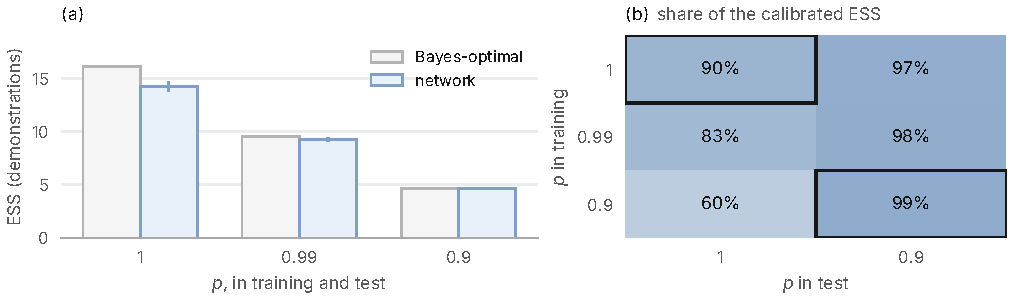
\includegraphics[width=\textwidth]{networks.pdf}
\caption[The ESS of a description to meta-trained networks]{\textbf{Networks come close to the Bayes-optimal ESS and take their trust in a description from training.} All panels use the specific description ($r = 0.01$), $d = 5$, $a_0 = 10$, and no demonstrations. Each network ESS shown is the mean over three networks trained with different random seeds, and the error bars show $\pm$ one standard deviation across them. (a) Networks trained and tested at the same reliability $p$. The bars show the Bayes-optimal ESS on the same prompts and the network's ESS, which is read from the network's own no-description curve. (b) Networks trained at one reliability and tested at another. Each cell shows the network's ESS as a share of the calibrated predictor's, and outlined cells mark cases where the training and test reliabilities match. Table~\ref{tab:networks} gives every value, including those for the loose description ($r = 0.1$).}
\label{fig:networks}
\end{figure}

\section{Results}\label{sec:net-results}
\paragraph{Networks come close to the Bayes-optimal ESS.} We first train and test each network at the same reliability (Figure~\ref{fig:networks}a). For the specific description at $p = 1$, the network's ESS is $14.3 \pm 0.5$ (mean $\pm$ standard deviation over three seeds). On the same prompts, the Bayes-optimal ESS is $16.1$. On $200{,}000$ prompts, it is $15.9$, close to the value $c + d + 1 = 16$ of Theorem~\ref{thm:reliable}(ii), since $c = 1/(r a_0) = 10$. At $p = 0.99$, the network's ESS is $9.3 \pm 0.2$, compared with $9.6$ for the Bayes-optimal predictor on the same prompts. At $p = 0.9$, it is $4.66 \pm 0.01$, compared with $4.63$. Because the three networks share their test prompts, these standard deviations reflect training alone and leave out the variation from prompts. We therefore compare each network with the Bayes-optimal predictor on the same prompts. Table~\ref{tab:networks} instead gives the Bayes-optimal ESS on $200{,}000$ prompts. At $p = 0.99$, that value ($8.96$) lies below the networks' mean ESS, whereas the Bayes-optimal ESS on the networks' own prompts ($9.6$) lies above it. A network's ESS can exceed the Bayes-optimal ESS on the same prompts, as it does at $p = 0.9$, because it is read from the network's own no-description curve rather than from the Bayes-optimal one. For the loose description, the network's ESS is within $0.1$ of the Bayes-optimal ESS at every reliability. At $p = 1$, for example, it is $5.85 \pm 0.03$, compared with $5.89$ (Table~\ref{tab:networks}).

\paragraph{ESS as demonstrations accumulate.} Figure~\ref{fig:networks-ess-n} shows each network's $\ess_n$ at its training reliability as demonstrations accumulate. The test prompts hold at most $20$ demonstrations, so the largest $\ess_n$ that can be read is $20 - n$. For the loose description, the networks' $\ess_n$ follows the Bayes-optimal $\ess_n$ to within $0.6$ at every $n$ the grid can show. For the specific description, the networks fall short of the Bayes-optimal $\ess_n$ by up to $2.4$ demonstrations at $p = 1$, $2.9$ at $p = 0.99$, and $1.4$ at $p = 0.9$. They exceed it by at most $0.3$. Both comparisons hold until the ESS can no longer be read within the grid. With five demonstrations in hand, the three networks trained at $p = 0.9$ have an ESS of $4.83$, $4.79$, and $4.77$, compared with $5.20$ for the Bayes-optimal predictor.

\begin{figure}[t]
\centering
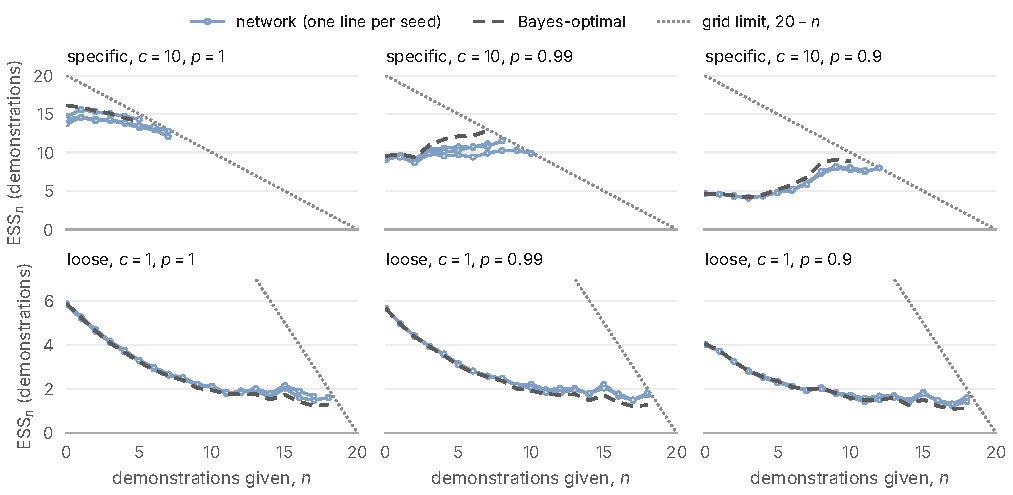
\includegraphics[width=\textwidth]{networks_ess_n.pdf}
\caption[The networks' ESS as demonstrations accumulate]{\textbf{The networks' ESS as demonstrations accumulate.} Each panel shows $\ess_n$ for the meta-trained networks, with one line per training seed, and for the Bayes-optimal predictor on the same prompts. The networks are trained and tested at the same reliability $p$. The top row uses the specific description ($r = 0.01$), and the bottom row uses the loose description ($r = 0.1$). Here $d = 5$ and $a_0 = 10$, and each network is tested on $20{,}000$ prompts. A curve stops where the error without the description would reach the error with it only after more than the $20$ demonstrations of the grid. The dotted line, $20 - n$, is the largest ESS that the grid can show.}
\label{fig:networks-ess-n}
\end{figure}

\paragraph{Training sets a network's trust.} With no demonstrations, the prompt carries no information about relevance (Section~\ref{sec:proof-unreliable}, Step~1). Any learner must therefore take its trust in a description from its training. The networks show how much of that trust they take (Figure~\ref{fig:networks}b). The networks trained at $p = 0.9$ keep hedging even when every test description is relevant. Their implied trust is $0.87$ to $0.89$ across the three seeds. Their ESS on reliable descriptions is $9.5 \pm 0.4$, whereas the calibrated predictor reaches $15.9$ and the trained one $10.8$.

The networks trained on specific descriptions at $p = 1$ or $p = 0.99$ treat every description as relevant when no demonstrations are shown. Their implied trust lies between $0.95$ and $1.02$, so the two training reliabilities cannot be told apart without demonstrations. Demonstrations separate them. On prompts in which one description in ten is irrelevant, the description lowers the error of the networks trained at $p = 0.99$ at every $n$, as it does for the Bayes-optimal predictor. It lowers their error by $3.5$ to $3.7$ with six demonstrations and by $0.08$ to $0.13$ with $20$. The networks trained at $p = 1$ instead trust the description fully. As Section~\ref{sec:trust} predicts, full trust costs little with no demonstrations. Their ESS is then $4.58 \pm 0.03$, compared with $4.70$ for the calibrated predictor. From six demonstrations on, however, their error is higher with the description than without it, in all three seeds. The fully trusting Bayes-optimal predictor behaves in the same way. With eight demonstrations, for example, the first of these networks has an error of $4.6$ with the description and $2.3$ without it.

\begin{table}[t]
\centering\small
\caption[The meta-trained networks against the Bayes-optimal predictors]{\textbf{The meta-trained networks against the Bayes-optimal predictors.} Here $d = 5$ and $a_0 = 10$, and each network is evaluated on $20{,}000$ prompts. Rows are grouped by training reliability, and ``Seeds'' gives the number of networks, trained with different random seeds, behind each row. ``Network'' is the mean ESS over these networks, $\pm$ the standard deviation across them; for a single network, it is $\pm$ the standard error over prompts. ``Trained'' and ``calibrated'' are the Bayes-optimal predictors that use the training and the test reliability, respectively, and they are shown once where the two coincide. Calibrated values, and trained values where the two reliabilities coincide, use $200{,}000$ prompts (standard errors at most $0.1$). Other trained values use the network's evaluation prompts. Prompt noise alone can move these values by up to $0.6$, so a trained value can exceed the calibrated one. ``Trust'' is the network's implied trust with no demonstrations, averaged over the networks in the row.}
\label{tab:networks}
\vspace{3pt}
\begin{tabular}{rrrcrrrr}
\toprule
& & & & \multicolumn{3}{c}{ESS} & \\
\cmidrule(lr){5-7}
$r$ & $p_{\mathrm{train}}$ & $p_{\mathrm{test}}$ & Seeds & Network & Trained & Calibrated & Trust \\
\midrule
0.1 & 1 & 1 & 2 & 5.85 $\pm$ 0.03 & 5.89 & --- & 0.964 \\
0.1 & 1 & 0.99 & 1 & 5.65 $\pm$ 0.06 & 5.66 & 5.61 & 0.991 \\
0.1 & 1 & 0.9 & 2 & 4.02 $\pm$ 0.03 & 3.98 & 4.10 & 0.964 \\
0.01 & 1 & 1 & 3 & 14.26 $\pm$ 0.48 & 15.91 & --- & 1.008 \\
0.01 & 1 & 0.99 & 2 & 9.38 $\pm$ 0.16 & 9.54 & 8.96 & 1.015 \\
0.01 & 1 & 0.9 & 3 & 4.58 $\pm$ 0.03 & 4.54 & 4.70 & 1.008 \\
\midrule
0.1 & 0.99 & 1 & 2 & 5.87 $\pm$ 0.01 & 5.88 & 5.89 & 0.963 \\
0.1 & 0.99 & 0.99 & 2 & 5.65 $\pm$ 0.01 & 5.61 & --- & 0.963 \\
0.1 & 0.99 & 0.9 & 2 & 4.02 $\pm$ 0.03 & 3.99 & 4.10 & 0.963 \\
0.01 & 0.99 & 1 & 3 & 13.28 $\pm$ 0.57 & 16.01 & 15.91 & 0.982 \\
0.01 & 0.99 & 0.99 & 3 & 9.25 $\pm$ 0.15 & 8.96 & --- & 0.982 \\
0.01 & 0.99 & 0.9 & 3 & 4.60 $\pm$ 0.04 & 4.56 & 4.70 & 0.982 \\
\midrule
0.1 & 0.9 & 1 & 2 & 5.67 $\pm$ 0.06 & 5.75 & 5.89 & 0.883 \\
0.1 & 0.9 & 0.99 & 1 & 5.51 $\pm$ 0.06 & 5.55 & 5.61 & 0.901 \\
0.1 & 0.9 & 0.9 & 2 & 4.03 $\pm$ 0.01 & 4.10 & --- & 0.883 \\
0.01 & 0.9 & 1 & 3 & 9.49 $\pm$ 0.44 & 10.79 & 15.91 & 0.876 \\
0.01 & 0.9 & 0.99 & 2 & 8.08 $\pm$ 0.28 & 8.55 & 8.96 & 0.880 \\
0.01 & 0.9 & 0.9 & 3 & 4.66 $\pm$ 0.01 & 4.70 & --- & 0.876 \\
\bottomrule
\end{tabular}

\end{table}

\section{Training Details}\label{sec:training}
Each demonstration token holds an input together with its label, and two indicator coordinates mark the token type. There is no positional encoding. The Transformer has $12$ layers, $8$ heads, and width $256$. It is trained with Adam (learning rate $10^{-4}$) for $40{,}000$ steps at batch size $1{,}024$, on fresh prompts at every step and without a curriculum. When a prompt has no description, the description token is masked out of attention. The prediction is read at the query token. The labels and the description are divided by $\sqrt{a_0}$ before they enter the network. Gradients are clipped to norm $1$, and training uses bfloat16 autocast. The number of demonstrations in a training prompt is uniform on $0$ to $20$ ($0$ to $15$ for the $r = 0.05$ and $r = 0.5$ networks described below).

Four further networks were trained once each, at $r = 0.5$ ($p = 1$ and $p = 0.9$) and at $r = 0.05$ ($p = 1$ and $p = 0.9$). Each reaches an ESS within $0.03$ of the Bayes-optimal ESS. The four values are $2.64$ compared with $2.66$, $2.16$ compared with $2.15$, $7.32$ compared with $7.35$, and $4.38$ compared with $4.37$.

\chapter{Pretrained Language Models}\label{ch:llm}

The meta-trained networks learn description statistics from repeated tasks. We next ask whether pretrained language models use the same information when it is stated explicitly. We use numerical mean estimation, a scalar version of the regression problem with fixed input $x=1$, following controlled tests of stated priors and in-context evidence \citep{gupta2025,akata2026}.

\section{Task and Evaluation}\label{sec:llm-task}

Each task has a hidden mean $w\sim\mathcal{N}(500,100^2)$ and demonstrations drawn from $\mathcal{N}(w,\sigma^2)$, with $\sigma=60$, then rounded to integers. A description supplies a value $m$ and uncertainty $\tau$, for example: ``Its mean was drawn from a normal distribution with mean 510 and standard deviation 30.'' The underlying Gaussian construction has $w\mid m\sim\mathcal{N}(m,\tau^2)$. We express precision in demonstration units as $c=\sigma^2/\tau^2$: stated standard deviations $60$, $30$, and $10$ correspond to $c=1$, $4$, and $36$.

We vary the stated precision, and add conditions stating a $50\%$ probability that the description is wrong. In these conditions the description remains relevant; the intervention tests how models respond to the stated probability. We also hold $m$ and the demonstrations fixed while describing a value generated at $c=36$ as having $c=4$. This isolates sensitivity to the stated uncertainty from sensitivity to the numerical value itself. Section~\ref{sec:llm-unreliability} includes genuinely irrelevant descriptions and evaluations under actual mixtures of relevant and irrelevant descriptions.

The main comparison uses the same $200$ tasks for five models with reasoning enabled and disabled: gpt-oss-20b \citep{openai2025}, Qwen3.5 9B \citep{qwen35}, Gemma~4 31B \citep{gemma4}, GPT-6 Sol, and Claude Opus~4.6. Claude Haiku~5.5 is evaluated with reasoning at medium effort. Checkpoints are held fixed within model, although serving environments and decoding settings differ for some comparisons. Sections~\ref{app:llm}--\ref{sec:llm-runs} report these details, response extraction, token limits, reruns, and a larger non-reasoning evaluation on $2{,}000$ tasks.

\paragraph{A reference based on the prompt.}
The prompt specifies the observation noise and description, but not the task generator's baseline prior. Our \emph{prompt-based Bayesian reference} therefore uses the stated description and a uniform fallback over the three-digit range. For a description asserted to be relevant, ignoring negligible boundary effects, its prediction is
\begin{equation}\label{eq:scalar-rule}
\hat w_{\mathrm{ref}}=\frac{c\,m+n\bar y}{c+n},
\end{equation}
where $\bar y$ is the demonstration mean. Under the continuous, correctly specified Gaussian model with a flat baseline prior, the description has exact ESS $c$. There is no random-design dimension term because every observation measures the same scalar mean.

Intuitively, the description counts as $c$ further demonstrations at $m$: it adds a precision of $1/\tau^2=c/\sigma^2$, equal to that of $c$ demonstrations. This is the conjugate normal model of Chapter~\ref{ch:background} with $n_0=c$, and the squared error is $\sigma^2/(c+n)$ with the description and $\sigma^2/n$ without it.

This reference follows the prompt even when a stated precision or reliability differs from the data generator. It is therefore a model of inference from the stated information, rather than an oracle for every evaluation condition. When the description may be wrong, its posterior also depends on the chosen fallback; we report sensitivity to that choice.

For each model, we compute ESS from its own demonstrations-only curve and summarize it by the median over $n\in\{1,2,4\}$. The same calculation gives reference ESS $34.6$ for $c=36$, rather than the idealized value $36$, because of finite-sample error and interpolation. We also regress predictions on $m$, $\bar y$, and an intercept. The coefficient on $m$ measures reliance on the description; the reference coefficient is $c/(c+n)$ when the description is asserted to be relevant.

\begin{figure}[htbp]
\centering
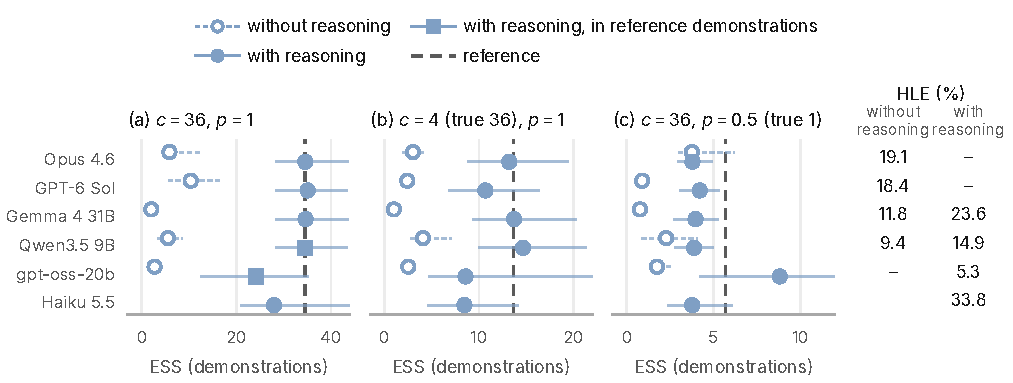
\includegraphics[width=\textwidth]{llm_ess.pdf}
\caption[Reasoning improves the use of stated precision, with model-specific exceptions]{\textbf{Reasoning improves the use of stated precision, with model-specific exceptions.} Summary ESS on $200$ tasks at $\sigma=60$: median over $n=1,2,4$, with paired $95\%$ bootstrap intervals over tasks. Open and filled points denote reasoning disabled and enabled; dashed and solid intervals distinguish the modes. Vertical dashed lines show the prompt-based Bayesian reference. (a) Relevant description with $c=36$: reference ESS $34.6$. (b) The same value, generated at $c=36$, is stated to have $c=4$: reference ESS $13.7$, because the value is more accurate than stated. (c) The description in (a) is assigned a $50\%$ probability of being wrong, while remaining relevant: reference ESS $5.7$ under the uniform fallback, which the prompt does not state. For GPT-6 Sol and Haiku~5.5, stating it changes which rule they follow but barely changes their ESS (Section~\ref{sec:llm-rules}). Square reasoning markers for Qwen3.5 9B in (a,b) and gpt-oss-20b in (a) use the reference's demonstrations-only curve because the models' own curves do not reach the crossing; these values are in reference-demonstration units. Haiku~5.5 uses medium effort. Intervals are clipped to the displayed range. HLE scores \citep{phan2025}, as reported by \citet{aa2026}, provide descriptive context; dashes indicate unavailable scores for the evaluated mode, and blanks indicate modes not evaluated.}
\label{fig:llm}
\end{figure}

\section{Reasoning and Stated Precision}\label{sec:once}\label{sec:reasoning}

\paragraph{Weak sensitivity without reasoning.}
For the $c=36$ description, non-reasoning ESS ranges from $1.5$ to $5.8$ across the five models, compared with $34.6$ for the reference (Figure~\ref{fig:llm}a). Models generally underweight this precise description and respond weakly when its stated precision changes. At $n=4$, GPT-6 Sol assigns weights $0.12$ and $0.13$ at stated $c=36$ and $c=4$, respectively, compared with reference weights $0.90$ and $0.50$. Opus~4.6 responds more, with weights $0.40$ and $0.20$. When the same value is described as $c=4$ instead of $c=36$, reference ESS falls from $34.6$ to $13.7$, whereas no model's ESS changes by more than $2.8$ (Figure~\ref{fig:llm}b).

\paragraph{Reasoning recovers precision weighting in several models.}
With reasoning enabled, Opus~4.6, GPT-6 Sol, and Gemma~4 31B reach approximately the reference ESS in both precision conditions; Haiku~5.5 at medium effort comes close. Among diagnostically separated tasks at $n=4$, the weight implied by an individual reply is within $0.05$ of the reference weight in $95$--$100\%$ of these models' replies (Section~\ref{sec:llm-rules}). This supports a change in how the description and demonstrations are combined, beyond an improvement in aggregate error alone.

Qwen3.5 9B and gpt-oss-20b also approach the reference precision weights, but arithmetic errors complicate their ESS. Their demonstrations-only curves can rise at larger $n$, preventing a crossing within the evaluated grid. For these cases, square markers in Figure~\ref{fig:llm} report sample equivalence using the reference's demonstrations-only curve, a different quantity from learner-specific ESS. Errors with the description also reduce gpt-oss-20b's ESS in some conditions. Reported HLE scores do not order these behaviors: some higher-scoring non-reasoning models use precision less accurately than lower-scoring reasoning models. This comparison is descriptive and does not isolate the mechanism responsible for the difference.

\section{Stated Reliability and Wording}\label{sec:llm-stated}

\paragraph{Reasoning models update relevance when the prompt says what a wrong description implies.}
Adding a stated $50\%$ probability of error lowers reference ESS from $34.6$ to $5.7$ under the uniform fallback. Without reasoning, no model's ESS falls by more than a factor of $2.7$, compared with a factor of about six for the reference. With reasoning, GPT-6 Sol, Gemma~4 31B, and Qwen3.5 9B closely track a different rule: they retain the stated relevance probability and weight $m$ by $p\,c/(c+n)$ (Table~\ref{tab:hedge}). This averages the relevant and irrelevant predictions using the \emph{prior} mixture weights.

Bayesian inference instead updates relevance by comparing how likely the demonstrations are if the description applies and if it does not. The prompt says only that the mean is then ``unknown'', which leaves the second likelihood, and so the update, undefined; keeping the stated probability is one defensible response. We therefore repeat the condition for GPT-6 Sol at low effort and Haiku~5.5 at medium effort, changing only the warning to say that the mean ``was instead drawn uniformly at random from the whole numbers 100 to 999'', the fallback the reference assumes. On tasks where the reference and fixed-rule predictions differ by at least $5$, the share of replies closer to the reference rises from $0$--$2\%$ to $89$--$97\%$ for GPT-6 Sol and from $21$--$41\%$ to $87$--$95\%$ for Haiku~5.5 (Section~\ref{sec:llm-rules}). Once the alternative is specified, both models update relevance from the demonstrations. The update is not always calibrated: with a stated $10\%$ chance, both rely on the description less than the reference does, and their ESS falls to about $18$, against $27.5$.

\paragraph{More explicit statistical descriptions are used more consistently.}
We test three alternative wordings with GPT-6 Sol and Haiku~5.5. Both closely follow Equation~\eqref{eq:scalar-rule} under the original wording and ``An earlier estimate put its mean at $m$, with a standard error of $\tau$.'' Under ``Its mean is about $m$, give or take $\tau$'' and ``Mean: $m\pm\tau$,'' they often return $m$ and disregard demonstrations. With the first informal wording, GPT-6 Sol skips reasoning in $24$--$51\%$ of replies per condition and usually returns $m$ in those replies. Haiku~5.5 returns $m$ in $71\%$ of the replies for which it does reason.

These alternatives preserve the numerical values but do not specify an equally precise statistical interpretation. The statistical wordings explain how the uncertainty should enter the task; informal uncertainty expressions leave that relationship less explicit. As with the unstated fallback, the finding therefore concerns the specificity of the description as a whole, including its instructions for interpreting uncertainty, rather than invariance to semantically equivalent phrasing.

\section{Additional Language-Model Results and Evaluation Details}\label{app:llm}

We generate $2{,}000$ tasks. Six open-weight models answer all tasks without reasoning; we refer to these experiments as the \emph{full run}. The models are gpt-oss-20b, Qwen3.5 9B, and Gemma~4 31B, which also appear in Sections~\ref{sec:llm-task}--\ref{sec:llm-stated}, together with Phi-4 (14B; \citealp{abdin2024}), OLMo~2 32B Instruct \citep{walsh2025}, and Gemma~4 12B. The experiments in Sections~\ref{sec:llm-task}--\ref{sec:llm-stated} use the first $200$ tasks. Unless stated otherwise, the results in this section and those that follow use the full run without reasoning.

Table~\ref{tab:llm} reports summary ESS, defined as the median over $n \in \{1,2,4\}$, with uncertainty intervals. Figure~\ref{fig:curves} shows the underlying learning curves. Tables~\ref{tab:llm-worth} and~\ref{tab:llm-worth-written}, in Appendix~\ref{app:llm-tables}, report ESS at every evaluated demonstration count; Table~\ref{tab:sensitivity} compares interpolation methods; Table~\ref{tab:llm-full}, also in Appendix~\ref{app:llm-tables}, reports description weights for the models with a distribution readout; and Table~\ref{tab:mixture} evaluates genuinely unreliable descriptions.

Throughout these sections, the \emph{prompt-based Bayesian reference} uses the probabilistic claims in the prompt together with an explicit assumption for the unspecified fallback prior. It is optimal under that assumed model. When the stated description differs from the data-generating process, it need not minimize error under the evaluation distribution. The reference labeled ``Bayes-optimal'' in the plots and tables has this meaning.

\section{Prompts, Tasks, and Model Readouts}

\paragraph{Model inclusion.}
We retain a model only if it produces a number in at least three quarters of replies overall and in at least half of replies without a description at each of $n = 1$, $2$, and $4$. The latter conditions determine the baseline curve used for summary ESS. This criterion excludes MiniCPM5~2B \citep{minicpm5}, OLMo~2 7B Instruct, and OLMo~2 13B Instruct, whose replies begin with a number in $62\%$, $20\%$, and $10\%$ of cases, respectively. These models often begin with explanations such as ``To predict\ldots'' or ``Given\ldots'' despite the numeric-only instruction. For example, OLMo~2 7B's summary ESS for the $c = 36$ description is $21$, but this value comes from a readout that rests on a minority of the model's probability.

The full run uses Hugging Face Transformers at each model's native precision, with checkpoints \nolinkurl{openai/gpt-oss-20b}, \nolinkurl{microsoft/phi-4}, \nolinkurl{allenai/OLMo-2-0325-32B-Instruct}, \nolinkurl{Qwen/Qwen3.5-9B}, \nolinkurl{google/gemma-4-12B-it}, and \nolinkurl{google/gemma-4-31B-it}. Tasks are sampled by a seeded generator. Reasoning is disabled where the chat template supports this option. For gpt-oss-20b, generation begins in the final channel, after the channel normally used for reasoning.

\paragraph{Distribution and written readouts.}
For gpt-oss-20b, Phi-4, and OLMo~2 32B without reasoning, the prediction is the mean of the first-token distribution over the $900$ three-digit number tokens. We call this the \emph{distribution readout}. These three models encode every three-digit integer as a single token, and we renormalize the first-token probabilities over these tokens. Other models, and all reasoning runs, use the number in the final answer, called the \emph{written readout}. We also evaluate written readouts for the three distribution-readout models as a robustness check (Tables~\ref{tab:llm} and~\ref{tab:paraphrase}). OLMo~2 32B assigns $41\%$ of first-token probability to numbers without a description at $n = 1$, and $75\%$ at $n = 2$. Its distribution readout at $n = 1$ therefore summarizes a minority of the first-token probability mass.

\begin{table}[htbp]
\centering\small
\setlength{\tabcolsep}{2.4pt}
\caption[Description ESS and weights in the full run without reasoning]{\textbf{Description ESS and weights in the full run without reasoning.} Left: median ESS over $n = 1$, $2$, and $4$, for relevant descriptions with $c = 1$, $4$, and $36$, and for the $c = 36$ description when irrelevant or accompanied by a stated $10\%$ or $50\%$ chance of being wrong. Brackets give $95\%$ bootstrap intervals. An upper bound, $\leq$, indicates that one demonstration alone outperforms the description-conditioned prediction. Right: the coefficient on the stated value at $n = 1$; the Bayesian reference weight is $c/(c+n)$. All results use $\sigma = 60$. ``Written'' denotes the written readout.}
\label{tab:llm}
\vspace{3pt}
\fittable{../../results/llm-test/llm_table.tex}
\end{table}

\paragraph{Prompt.}
The following text is supplied as the user turn in the model's chat template:
\begin{quote}\scriptsize\ttfamily\raggedright
The numbers below are drawn from a normal distribution with standard deviation 60.\\
Its mean was drawn from a normal distribution with mean 510 and standard deviation 30.\\[3pt]
548\\
431\\[3pt]
Predict the next number. Reply with the number only.
\end{quote}

Without a description, the second sentence is ``Its mean is unknown.'' To state unreliability, a third sentence is added: ``There is a 10\% chance that this statement is wrong, in which case the mean is unknown.'' In the rerun of Section~\ref{sec:llm-stated} that states the fallback, its last clause becomes ``in which case the mean was instead drawn uniformly at random from the whole numbers 100 to 999.'' With no demonstrations, the final question is ``Predict the first number.''

\paragraph{Task generation.}
A relevant description value is sampled conditional on the task so that the joint distribution satisfies $m \sim \mathcal{N}(500,100^2-\tau^2)$ and $w\mid m \sim \mathcal{N}(m,\tau^2)$. A task is redrawn if a displayed number or description value falls outside $100$ to $999$; this occurs for less than $1\%$ of tasks. The full run also includes $\sigma = 30$ conditions. Both standard deviations stated in the prompt are then halved, preserving $c \in \{1,4,36\}$. The qualitative pattern is unchanged (Table~\ref{tab:llm-worth}).

\paragraph{Numeric response rates.}
For the distribution readout, the numeric response rate is the probability mass assigned to number tokens at the first position. For the written readout, it is the fraction of replies containing a three-digit number. Tables~\ref{tab:paraphrase}, \ref{tab:llm-worth}, \ref{tab:llm-worth-written}, and~\ref{tab:llm-full} report this quantity as ``number''. Tables~\ref{tab:paraphrase} and~\ref{tab:llm-full} italicize cells whose rate is below three quarters.

\paragraph{Written-readout implementation and checks.}
The written readout extracts the first number with three digits before an optional decimal part and retains the decimals. Without reasoning, decoding is greedy with a limit of eight new tokens. Those predictions were recorded using an earlier readout that retained only the integer part; this rarely changes the value because decimal outputs are uncommon. With reasoning, extraction is applied to the final answer. Replies without a qualifying number are excluded from both error curves and weight regressions.

For gpt-oss-20b, written-readout weights differ from distribution-readout weights by at most $0.21$ across all conditions and demonstration counts. For $c = 1$, $4$, and $36$, written-readout summary ESS is $0.2$, $2.0$, and $3.7$, compared with $0.9$, $2.0$, and $2.8$ from the distribution readout. A single greedy response is a noisier summary than the distribution mean. Phi-4 produces a number in only $63\%$ of written replies across all conditions, so Table~\ref{tab:llm} reports only its distribution readout. In the wording experiment, however, its numeric response rate exceeds three quarters for the original wording. OLMo~2 32B produces a number in only $5\%$, $36\%$, and $48\%$ of written replies without a description at $n = 1$, $2$, and $4$, respectively, with $\sigma = 60$; we therefore do not report its written-readout ESS. Its written-readout weights for the three relevant descriptions at $n = 1$ are $0.83$, $0.81$, and $0.83$, compared with distribution-readout weights of $0.72$, $0.70$, and $0.70$.

\section{ESS Estimation and the Bayesian Reference}

\paragraph{Measurement.}
We apply Definition~\ref{def:ess} to squared error against the hidden mean. In the full run, the baseline curve is evaluated at $n = 1$, $2$, $4$, $\ldots$, $64$. We interpolate squared error, rather than its square root, linearly in $\log n$. The ESS at $n$ is the first interpolated demonstration count $t$ that matches the description-conditioned error, minus $n$.

If the description-conditioned error lies below the entire baseline curve up to $t_{\max}$, we report $\ess_n > t_{\max}-n$. Because the curve starts at one demonstration, we report $\ess_n \leq 1-n$ when one demonstration alone already gives lower error. Summary ESS uses $n = 1$, $2$, and $4$. We exclude $n = 0$ because models rarely return a number without a description or demonstrations. At large $n$, ESS is strongly affected by slow baseline learning and excessive weight on the $c = 1$ and $c = 4$ descriptions. At $\sigma = 60$ and $n = 64$, model root-mean-square error ranges from $9$ to $23$, compared with $7.5$ for the reference. A learner with a flatter baseline curve can assign a larger ESS to the same error reduction. Description-weight estimates complement ESS because they do not use that curve.

Bootstrap replicates resample tasks jointly for the description-conditioned and baseline curves and recompute the complete ESS statistic. The intervals therefore measure variation across tasks; they do not include interpolation bias, quantified below.

\paragraph{Reference prior and exact sample equivalence.}
The prompt-based Bayesian reference takes ``unknown'' to mean uniform over $100$ to $999$. Without a description, its prediction is therefore approximately the demonstration mean, with negligible boundary truncation for the evaluated prompts. For a relevant Gaussian description, the idealized continuous model with a flat baseline prior has exact sample equivalence $c$. Integer rounding, finite-range truncation, and the task-rejection rule are not part of that exact identity; we compute the reported reference values on the same generated tasks as the models. When a chance of being wrong is stated, the reference uses it as a prior probability of irrelevance and updates that probability from the demonstrations. Otherwise, it treats the description as relevant.

Applying the empirical ESS procedure to the full-run reference gives $1.3$, $4.4$, and $36$ for $c = 1$, $4$, and $36$ at $\sigma = 60$, and $1.2$, $4.7$, and $43$ at $\sigma = 30$. Interpolation in $\log n$ induces an upward bias, while finite-task sampling can shift the estimate in either direction. We use the same estimator for the reference and the models. On the $200$ tasks of Sections~\ref{sec:llm-task}--\ref{sec:llm-stated}, the grid additionally includes $n = 40$ and $48$ near the $c = 36$ crossing, and the reference values are $1.0$, $3.5$, and $34.6$.

The actual task prior, $\mathcal{N}(500,100^2)$, is not stated in the prompt. A reference using that prior would have baseline precision equivalent to $0.36$ demonstrations at $\sigma = 60$ and $0.09$ at $\sigma = 30$. At $\sigma = 60$, the corresponding idealized continuous Gaussian model would give a relevant description exact ESS $c-0.36$, namely $0.64$, $3.64$, and $35.64$. This is the scalar analogue of $(1-r)c$ in Chapter~\ref{ch:specificity}, with $r=\tau^2/100^2$. We use the prompt-based reference because the models are not given the actual task prior. This distinction matters under misspecification: unlike the correctly specified Bayesian predictor in Chapters~\ref{ch:specificity}--\ref{ch:reliability}, a reference that accepts an incorrect description can have negative ESS, indicating increased prediction error \citep{reimherr2021}.

\paragraph{Sensitivity to interpolation.}
The full-run grid doubles $n$, so interpolation can affect ESS. On the reference's idealized errors, $\sigma^2/n$ without a description and $\sigma^2/(c+n)$ with one, interpolation in $\log n$ overestimates ESS by $0.2$, $0.3$, and $1.8$ for $c = 1$, $4$, and $36$. Linear interpolation in $n$ gives overestimates of $0.3$, $0.6$, and $4.1$.

For the models without reasoning, the relevant crossings are unique. Among the twelve baseline curves across the two noise levels, only Phi-4 at $\sigma = 60$ increases, slightly, from $20.3$ at $n = 32$ to $20.4$ at $n = 64$. Table~\ref{tab:sensitivity} compares four estimators: interpolation in $\log n$; linear interpolation in $n$; a least-squares non-increasing fit using pool adjacent violators; and a relative-least-squares fit of $A/(n+n_0)+B$ to the baseline errors. The final form is a Bayesian learning curve plus an error floor and recovers exact ESS when fit to the reference's idealized errors.

Across these choices, no model's summary ESS changes by more than $1.4$ demonstrations. For the $c = 36$ description, no model exceeds $8.1$, while the reference ranges from $35$ to $38$. Differences become larger at higher demonstration counts, where a flat learning curve turns a small error difference into a large change in ESS. For example, gpt-oss-20b at $n = 8$ and $c = 36$ has ESS $17$ under the estimator in Table~\ref{tab:llm-worth}, but $9.2$ under the fitted curve.

\begin{figure}[htbp]
\centering
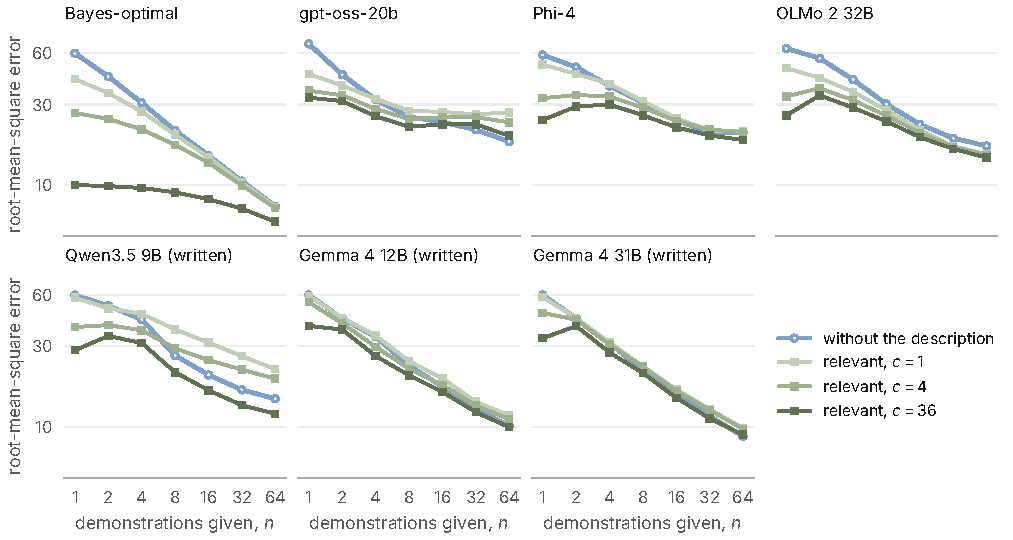
\includegraphics[width=\textwidth]{llm_curves.pdf}
\caption[Learning curves used to estimate language-model ESS]{\textbf{Learning curves used to estimate language-model ESS.} Root-mean-square error versus demonstration count for the reference and six models in the full run without reasoning, at $\sigma = 60$. Blue curves omit the description; green curves use relevant descriptions, with darker shades indicating higher $c$. Replies without a number are excluded. ESS is the horizontal distance from the description-conditioned point at $n$ to the baseline curve at the same error. For four models, error with $c = 36$ increases between one and two demonstrations because the models shift toward the observations more than the reference does (Table~\ref{tab:llm-full}).}
\label{fig:curves}
\end{figure}

\begin{table}[htbp]
\centering\small
\setlength{\tabcolsep}{4pt}
\caption[Sensitivity of summary ESS to baseline-curve estimation]{\textbf{Sensitivity of summary ESS to baseline-curve estimation.} Median ESS over $n = 1$, $2$, and $4$ for relevant descriptions, using the full run without reasoning at $\sigma = 60$. ``Log $n$'' is the primary estimator; ``linear'' interpolates in $n$; ``monotone'' applies a non-increasing fit; and ``fit'' uses $A/(n+n_0)+B$. The reference's idealized ESS values are $1$, $4$, and $36$.}
\label{tab:sensitivity}
\vspace{3pt}
\fittable{../../results/llm-test/llm_table_sensitivity.tex}
\end{table}

\section{Results of the Full Run}\label{sec:llm-full-run}

\paragraph{Summary ESS.}
Across the six models, the $c = 36$ description has summary ESS $1.4$ to $7.6$, compared with reference ESS $36$ on these tasks, and ESS at most $15$ at any of $n = 1$, $2$, and $4$ (Table~\ref{tab:llm}). The $c = 1$ and $c = 4$ descriptions have summary ESS $0.0$ to $1.9$ and $0.2$ to $4.1$, compared with $1.3$ and $4.4$. ESS rises with $c$ mainly because a more specific description has a value closer to the task, as Table~\ref{tab:control} shows.

\paragraph{Description weights.}
At $\sigma = 60$, with no demonstrations and no stated reliability, the models return the description value (weight $0.92$ to $1.10$), although Phi-4 and OLMo~2 32B then begin only $20$ to $23\%$ and $50$ to $59\%$ of their replies with a number. At $n = 1$, the weight of gpt-oss-20b, Phi-4, and OLMo~2 32B changes by at most $0.08$ from $c = 1$ to $c = 36$, and if anything falls, whereas the reference weight rises from $0.50$ to $0.80$ to $0.97$ (Table~\ref{tab:llm}). At every $n$ from $1$ to $64$ and at both noise levels, the spread of these three models' weights across $c$ is at most $0.16$, compared with a reference spread of $0.34$ to $0.71$ (Table~\ref{tab:llm-full}). The weights of the two Gemma models do rise with $c$, by about $0.25$ between $c = 1$ and $c = 36$ at $n = 1$, half the reference rise. The weight of Qwen3.5 9B does not. Models therefore underweight a precise description and, with many demonstrations, overweight the least precise one. At $n = 64$, gpt-oss-20b still assigns weight $0.23$ to the $c = 1$ value, compared with reference weight $0.02$, and that description raises its error (ESS $-57$).

\paragraph{Stated unreliability.}
A stated $10\%$ or $50\%$ chance of being wrong leaves the ESS of gpt-oss-20b and OLMo~2 32B about where it was, and Phi-4's ESS even rises, from $7.6$ to $8.7$ and $9.7$. Qwen3.5 9B and Gemma~4 31B have lower ESS, but by about as much for $50\%$ as for $10\%$. Gemma~4 12B's ESS falls at $10\%$ and rises at $50\%$ (Table~\ref{tab:llm}). No model's ESS falls in proportion to the stated probability, whereas reference ESS falls to $22$ and $5.8$.

\section{Unreliability, Description Accuracy, and Wording}\label{sec:llm-unreliability}

\paragraph{Irrelevant descriptions.}
An irrelevant description uses the value from a different, independently sampled task. At $c = 36$, these descriptions have negative ESS for every model and for the prompt-based reference, which treats them as relevant. The models assign less weight to the description and consequently incur lower error in this condition: at $n = 4$, their root-mean-square errors range from $35$ to $64$, compared with $124$ for the reference. Also at $n = 4$, their weight on an irrelevant $c = 36$ value is $0.01$ to $0.33$, compared with $0.18$ to $0.44$ on a relevant one.

\paragraph{Actual unreliability.}
The stated-unreliability experiments keep descriptions relevant and vary what models are told. Table~\ref{tab:mixture} instead evaluates the mixture in Chapter~\ref{ch:setup}. We combine squared errors from the relevant and irrelevant conditions, on the same tasks, with weights $p$ and $1-p$, and then estimate ESS. We evaluate models both with and without disclosure of the irrelevance probability. The fully trusting reference always treats the description as relevant; the calibrated reference starts from irrelevance probability $1-p$ and updates it from the observations.

At actual reliability $p = 0.9$, a $c = 36$ description has ESS $5.5$ for the calibrated reference and $0.2$ for the fully trusting reference. Model ESS ranges from $0.4$ to $3.2$ when the reliability is not stated and from $-0.1$ to $4.0$ when it is stated. Model weights depend weakly on $p$, and stating the probability changes ESS by at most two demonstrations in either direction. Their nearly fixed weight on the description thus acts as a hedge between full trust and calibration. At $p = 0.5$, the description is worth less than one demonstration to the calibrated reference and at most one to every model.

\begin{table}[htbp]
\caption[Description ESS under actual unreliability]{\textbf{Description ESS under actual unreliability.} Relevant and irrelevant $c = 36$ conditions are combined with weights $p$ and $1-p$. Results are summary ESS with $95\%$ task-bootstrap intervals for the full run without reasoning at $\sigma = 60$. The fully trusting reference assumes relevance; the calibrated reference uses the actual reliability and updates it from demonstrations. A bound indicates that one demonstration alone outperforms the description-conditioned prediction at one or more summary demonstration counts.}
\label{tab:mixture}
\centering\footnotesize
\fittable{../../results/llm-test/llm_table_mixture.tex}
\end{table}

\paragraph{Wording without reasoning.}
We repeat the three relevant-description conditions and the no-description baseline at $n = 1$, $2$, and $4$ using three alternative description sentences: ``Its mean is about $m$, give or take $\tau$.'', ``Mean: $m \pm \tau$'', and ``An earlier estimate put its mean at $m$, with a standard error of $\tau$.'' Table~\ref{tab:paraphrase} uses the full-run tasks and written readouts.

Wording substantially changes the weight assigned to the description. For Gemma~4 12B with $c = 1$ and $n = 1$, this weight is $0.34$ under the original wording and $1.00$ under each alternative. For gpt-oss-20b, it ranges from $0.17$ to $0.67$. A coefficient above $1$ means that predictions vary more strongly with the stated value than the value itself. Nevertheless, none of the tested wordings yields the reference's sensitivity to specificity: across models and wordings, the weight difference between $c = 36$ and $c = 1$ is at most $0.25$ at $n = 1$ and $0.44$ at $n = 4$, compared with reference differences of $0.47$ and $0.70$. The informal descriptions do not uniquely specify a probability distribution, so this comparison also varies how precisely the task is specified.

\begin{table}[htbp]
\centering\footnotesize
\caption[Description weights under four wordings without reasoning]{\textbf{Description weights under four wordings without reasoning.} Weights are reported for the three relevant descriptions at $n = 1$ and $4$, using written readouts on the full-run tasks. ``Number'' denotes the numeric response rate; italics mark rates below three quarters. The reference weights are $0.50$, $0.80$, and $0.97$ at $n = 1$, and $0.20$, $0.50$, and $0.90$ at $n = 4$. Wording changes overall reliance on the description, but the observed change with stated specificity remains smaller than the reference change.}
\label{tab:paraphrase}
\vspace{3pt}
\fittable{../../results/llm-test/llm_table_paraphrase.tex}
\end{table}

\paragraph{Separating stated specificity from description accuracy.}
For each task, we take a description value generated either at $c = 36$ or at $c = 1$ and present it with each stated specificity in $\{1,4,36\}$. The tasks and demonstrations match the full run, and the experiment includes its own no-description prompts at every $n$ (Table~\ref{tab:control}). Repeated conditions reproduce the full run exactly except for gpt-oss-20b. Its distribution readout changes by a median of $0.8$ to $1.2$ across conditions, with a maximum difference of $39$; its written replies change in $12\%$ of cases, with median difference $0$. A newer library version is a possible explanation.

The prompt-based reference accepts the stated specificity. A value generated at $c = 1$ but stated as $c = 36$ therefore has reference ESS of about $-0.8$; a model that discounts the stated specificity can outperform it in that misspecified condition. For models without reasoning, description accuracy primarily determines ESS. When the value is generated at $c = 1$, each model's ESS remains between $-0.1$ and $2.0$ across all stated specificities. When the value is generated at $c = 36$, each model's ESS is higher, but from stated $c = 1$ to stated $c = 36$ it rises by at most $1.2$, whereas reference ESS rises from $2.5$ to $36$. For example, gpt-oss-20b has ESS $2.7$, $2.6$, and $2.8$ at stated $c = 1$, $4$, and $36$. Phi-4's ESS even falls, from $12$ at stated $c = 1$ to $7.6$ at stated $c = 36$, the reverse of the reference order.

\begin{table}[htbp]
\centering\small
\setlength{\tabcolsep}{4pt}
\caption[Sensitivity to stated specificity with the value and demonstrations held fixed]{\textbf{Sensitivity to stated specificity with the value and demonstrations held fixed.} Results use $\sigma = 60$, the full-run tasks, and the readout conventions of Table~\ref{tab:llm}. For a value generated at $c = 36$, the table reports its weight at $n = 1$ and summary ESS under each stated $c$. Results for the $200$-task runs of Sections~\ref{sec:llm-task}--\ref{sec:llm-stated} appear in Table~\ref{tab:reason}.}
\label{tab:control}
\vspace{3pt}
\fittable{../../results/llm-test/control_table.tex}
\end{table}

\section{Reasoning Runs and Execution Settings}\label{sec:llm-runs}

\paragraph{Shared evaluation prompts.}
Every model in Figure~\ref{fig:llm}, as well as Olmo~3 7B Think \citep{olmo2025three}, is evaluated on the same $7{,}800$ prompts from the first $200$ tasks. These include no-description prompts at $n = 1$, $2$, $4$, $\ldots$, $64$, with additional points at $n = 40$ and $48$ near the $c = 36$ crossing, and every description condition at $n = 1$, $2$, and $4$. The gpt-oss-20b run omits the two additional points and contains $7{,}400$ prompts. Results without reasoning for the open-weight models are taken from the full run restricted to these tasks. The two modes receive the same prompts, although their serving environments can differ as detailed below. At least $99.7\%$ of replies in each run contain a number.

\paragraph{Open-weight reasoning models.}
With reasoning, gpt-oss-20b runs in vLLM using greedy decoding, low reasoning effort, and at most $4{,}096$ new tokens. It reaches the final channel in $99.9\%$ of replies and uses $322$ tokens on average, and at least $97\%$ of replies reach it in every cell. An earlier run with a limit of $384$ tokens finished only $28$ to $54\%$ of the replies in the stated-reliability conditions, and the difference between a stated $10\%$ and $50\%$ that this run seemed to show came from which replies finished. Qwen3.5 9B runs through OpenRouter at temperature $0$, with reasoning enabled and a limit of $24{,}576$ new tokens. We pin requests to DeepInfra, which serves the model in bf16, because quantization varies across providers. Of its replies, $2{,}305$ loop to the token limit, a failure its model card warns of. Each is rerun once using the model card's recommended reasoning sampling settings (temperature $1.0$, top-$p$ $0.95$, top-$k$ $20$, presence penalty $1.5$); $10$ remain unfinished.

Gemma~4 31B (\texttt{gemma-4-31b-it}) runs through the Gemini API at temperature $0$. Reasoning is enabled by default, and the model uses $2{,}613$ reasoning tokens on average, with the same $24{,}576$-token limit. Of its replies, $435$ reach the limit; all finish after one rerun using the model card's recommended sampling settings (temperature $1.0$, top-$p$ $0.95$, top-$k$ $64$).

Olmo~3 7B Think runs in vLLM with greedy decoding and at most $32{,}768$ new tokens, the limit its model card recommends; at $8{,}192$ tokens, only $12$ of $20$ pilot replies finished. We rerun the $169$ replies that reach this limit once with temperature $0.6$ and top-$p$ $0.95$; $17$ remain unfinished. The model uses $9{,}215$ reasoning tokens on average. Its long greedy outputs are sensitive to hardware: an earlier stated-specificity run on a different GPU produces the same final number on only half the prompts. We therefore report one run. Despite its extensive reasoning, this model learns little from the demonstrations; its prediction behavior is reported below.

\paragraph{Models served through command-line agents.}
GPT-6 Sol (\texttt{gpt-6-sol}) runs through the Codex command-line agent under a subscription, in a read-only sandbox. We evaluate reasoning disabled, with no reasoning tokens, and reasoning enabled at low effort. The agent's instructions and tool definitions surround the prompt, much as a provider's system prompt surrounds a prompt sent through an API. The model invokes a shell command in $544$ replies with reasoning and $616$ without reasoning. Almost all such calls average demonstrations in no-description prompts with at least eight observations; other prompts account for seven calls with reasoning and $97$ without it. Improving the baseline error curve through these calculations lowers the ESS inferred from that curve. Tool use therefore does not inflate ESS through a weaker baseline, although access to tools remains a difference between this execution environment and tool-free runs.

Claude Opus~4.6 and Haiku~5.5 run through the Claude Code command line under a subscription, with one prompt per call, no tools, no project or user instructions, and a one-line system prompt. Opus~4.6 uses high effort in both evaluated modes, with reasoning either enabled or disabled; the disabled mode emits no reasoning tokens. When enabled, it reasons before at least $99\%$ of replies in each description condition and averages $599$ reasoning tokens across all replies. Without a description, it reasons before only $1\%$, $24\%$, and $79\%$ of replies at $n = 1$, $2$, and $4$, respectively. Haiku~5.5 (\texttt{claude-haiku-5-5}) is evaluated at medium and low effort, using the command line's default sampling temperature. At medium effort, it reasons before $37$ to $88\%$ of replies at $n = 1$ across conditions and before nearly all replies from $n = 2$ onward, with $270$ reasoning tokens on average. Its no-description error stays close to the reference through $n = 48$; at $n = 16$, for example, it is $15.8$ against $14.8$, with two replies far off. Its error rises at $n = 64$, where it divides the sum by $60$ instead of $64$ in $9$ of $200$ replies.

\paragraph{Interpreting the comparison between modes.}
The experiments hold the model checkpoint and prompts fixed within each paired comparison, but reasoning settings, serving software, readout, retry policy, and access to calculation tools are not uniform across all runs. The results describe the behavior of the evaluated configurations. They do not by themselves isolate a single internal mechanism responsible for the difference between modes.

\paragraph{ESS when baseline arithmetic fails.}
With reasoning, gpt-oss-20b and Qwen3.5 9B assign approximately the reference weight to the description: at $n = 4$ and $c = 36$, their weights are $0.89$ and $0.90$, compared with $0.90$ for the reference. However, both make errors when averaging longer demonstration sequences. Qwen3.5 9B has no-description root-mean-square error $15.1$ at $n = 16$ and $35.4$ at $n = 32$, compared with reference errors $14.8$ and $10.0$. From $n = 32$ onward, between $4$ and $24$ replies per cell differ from the sample mean by more than $20$; one reply gives $945$ for numbers averaging $467$.

For these models, the baseline curve rises after $16$ demonstrations, and some description-conditioned errors never meet it within the evaluated grid. Table~\ref{tab:reason} therefore also reports, in parentheses, a comparison using the Bayesian reference's baseline curve. This quantity is the number of demonstrations required by the reference without a description to match the model's error, rather than ESS in the model's own units. The gpt-oss-20b model also makes arithmetic errors with descriptions, reducing the reported ESS in those conditions; for example, it obtains $1.3$ when the prompt states a $10\%$ chance of being wrong. About $2\%$ of its replies are more than $40$ from the reference prediction, from errors such as exchanging the two variances. On the reference's baseline, its $c = 36$ description is therefore worth $24$ demonstrations, well below the reference's $34.6$, although its weight is right. A fitted weight hides such errors, whereas ESS does not.

Opus~4.6 and GPT-6 Sol do not exhibit these arithmetic failures. Opus~4.6 has root-mean-square error $7.4$ at $n = 64$, matching the reference on these tasks, and using either baseline gives the same ESS for these two models. At low effort, Haiku~5.5 often skips reasoning and repeats the demonstration. Its description weight at $n = 1$ is consequently low even in conditions whose ESS is close to the reference value.

\begin{table}[htbp]
\centering\small
\setlength{\tabcolsep}{2.5pt}
\caption[Description ESS across reasoning configurations]{\textbf{Description ESS across reasoning configurations.} Results use the first $200$ tasks at $\sigma = 60$. Summary ESS is computed using each run's baseline curve; parentheses show the value using the Bayesian reference's baseline where it differs. ``10\% wrong'' and ``50\% wrong'' denote the stated probability for a $c = 36$ description. The last column uses a value generated at $c = 36$ but described as $c = 4$. ``Reasoning'' identifies the mode and provider effort setting. An upper bound, $\leq$, indicates that one demonstration alone gives lower error; $>60$ denotes a crossing beyond the grid. Reference values use the same tasks and estimator. Olmo~3 7B Think's no-description error never drops below its error at one demonstration, so its reported crossings require particular caution; using the reference baseline gives a different comparison rather than resolving the weak model baseline.}
\label{tab:reason}
\vspace{3pt}
\fittable{../paper/tables/reason_table.tex}
\end{table}

\section{Prediction Rules and Reliability Updating}\label{sec:llm-rules}

\paragraph{Rules inferred from individual replies.}
A weight fitted across tasks can mix replies that follow different rules. At $n = 4$, we estimate the description weight implied by an individual prediction as $(\hat y-\bar y)/(m-\bar y)$. We use the $61$ tasks per cell where $|m-\bar y|\geq30$ and exclude replies without a number. We classify a reply as consistent with a rule if its implied weight is within $0.05$ of that rule's weight. The candidate weights are the Bayesian reference ($0.90$ for $c = 36$ and $0.20$ for $c = 1$); the reference with its two precisions exchanged ($0.10$ and $0.80$); the description counted as one additional observation, $1/(n+1)$; the description alone, with weight $1$; and the demonstrations alone, with weight $0$. The one-additional-observation rule coincides with the reference at $c = 1$.

With reasoning, Opus~4.6, GPT-6 Sol, Gemma~4 31B, and Haiku~5.5 match the reference rule on $95$ to $100\%$ of eligible replies. Without reasoning, $79\%$ of Opus~4.6 replies at $c = 36$ match none of these candidate rules, as do more than half of GPT-6 Sol replies. Olmo~3 7B Think instead repeats the description value in $96$ to $97\%$ of replies at $n = 1$, regardless of stated specificity. At $n = 4$, $70$ to $77\%$ of its replies match none of the rules, and only $3$ to $8\%$ match the reference. From task to task, it predicts the description value, the demonstration mean, or an invented pattern, and it makes arithmetic errors. Its no-description root-mean-square error remains near $55$ from $n = 1$ to $32$, compared with reference error $10$ at $n = 32$. Reasoning mode is therefore not sufficient for the desired behavior in every tested model.

Within each cell, Haiku~5.5's replies split by whether it reasons. At $n = 1$, replies with reasoning assign weights $0.50$, $0.80$, and $0.97$ to the relevant $c = 1$, $4$, and $36$ values, the reference weights to two decimals, at either effort. Replies without reasoning assign weight $0.00$ to $0.05$ and repeat the demonstration. Its overall weight at $n = 1$ mixes the two kinds of reply: $0.44$, $0.66$, and $0.74$ at medium effort. On these three descriptions, it reasons before $34$ to $53\%$ of replies at low effort, against $72$ to $82\%$ at medium effort, so its overall weight at $n = 1$ is lower at low effort and nearly flat, at $0.36$, $0.34$, and $0.41$. With more demonstrations it reasons more often, and its weight approaches the reference again: at $n = 4$ and low effort, it is $0.17$, $0.48$, and $0.86$, compared with $0.20$, $0.50$, and $0.90$. The choice to reason is the model's own, so this split describes its replies rather than the result of an experiment.

\paragraph{A fixed reliability rule.}
Table~\ref{tab:hedge} reports description weights for $c = 36$ when the prompt states a probability of being wrong. A predictor that combines the description-conditioned and no-description predictions with fixed weights $p$ and $1-p$ assigns weight $p\,36/(36+n)$ to $m$. Under the original warning, which leaves the fallback unstated, GPT-6 Sol, Gemma~4 31B, and Qwen3.5 9B with reasoning are close to this fixed rule. Opus~4.6 and Haiku~5.5 at medium effort fall below the reference weight by $n = 4$. Haiku~5.5 at low effort, which often skips reasoning at $n = 1$, comes closest to the reference weight. gpt-oss-20b assigns nearly the weight of a reliable description whatever the stated probability. These are behavioral comparisons; they do not identify the internal procedure used in every reply.

\paragraph{Sensitivity to the unspecified fallback prior.}
The prompt states only that, if the description is wrong, ``the mean is unknown''. A Bayesian relevance update compares the likelihood of the observations under the description with their likelihood under this fallback. Because the prompt leaves the fallback distribution unspecified, it does not determine a unique Bayesian relevance update.

For the $c = 36$ description with a stated $50\%$ chance of being wrong, the reference's fitted weights on the first $200$ tasks at $n = 1$, $2$, $4$, $8$, and $16$ are $0.58$, $0.61$, $0.64$, $0.58$, and $0.54$ with the uniform fallback over $100$ to $999$. They are $0.49$, $0.49$, $0.53$, $0.49$, and $0.45$ with the actual task prior $\mathcal{N}(500,100^2)$; $0.52$, $0.54$, $0.58$, $0.53$, and $0.49$ with $\mathcal{N}(500,200^2)$; and $0.72$, $0.74$, $0.74$, $0.67$, and $0.60$ with a uniform fallback over $0$ to $2{,}000$. The fixed rule gives $0.49$, $0.47$, $0.45$, $0.41$, and $0.35$.

By four demonstrations, the reference weight exceeds the fixed-rule weight for every fallback examined. Thus the observed agreement of several models with the fixed rule persists across these choices of reference. The size of their departure from Bayesian updating depends on the fallback, however; under the actual task prior, the reference update is small before four demonstrations.

\begin{table}[htbp]
\centering\small
\setlength{\tabcolsep}{3pt}
\caption[Description weights under stated unreliability]{\textbf{Description weights under stated unreliability.} Coefficients on the $c = 36$ description value for the first $200$ tasks, with stated irrelevance probability $1-p$. ``Fixed'' uses weight $p\,36/(36+n)$; the reference updates relevance using the uniform fallback over $100$ to $999$. Bootstrap standard errors are at most $0.03$ at $n = 4$ in the stated-$50\%$ condition, and at most $0.06$ overall, except for gpt-oss-20b, whose maximum is $0.09$. Several reasoning configurations closely track the fixed rule.}
\label{tab:hedge}
\vspace{3pt}
\begin{tabular}{lcccccc}
\toprule
& \multicolumn{3}{c}{$50\%$ wrong} & \multicolumn{3}{c}{$10\%$ wrong} \\
\cmidrule(lr){2-4} \cmidrule(lr){5-7}
& $n = 1$ & $2$ & $4$ & $1$ & $2$ & $4$ \\
\midrule
Reference & $0.58$ & $0.61$ & $0.64$ & $0.88$ & $0.87$ & $0.84$ \\
Fixed & $0.49$ & $0.47$ & $0.45$ & $0.88$ & $0.85$ & $0.81$ \\
\midrule
GPT-6 Sol & $0.50$ & $0.48$ & $0.45$ & $0.92$ & $0.88$ & $0.82$ \\
Opus~4.6 & $0.56$ & $0.43$ & $0.40$ & $0.93$ & $0.86$ & $0.77$ \\
Gemma~4 31B & $0.49$ & $0.46$ & $0.45$ & $0.89$ & $0.68$ & $0.76$ \\
Qwen3.5 9B & $0.50$ & $0.46$ & $0.43$ & $0.88$ & $0.84$ & $0.74$ \\
Haiku~5.5, medium & $0.55$ & $0.56$ & $0.46$ & $0.79$ & $0.93$ & $0.89$ \\
Haiku~5.5, low & $0.49$ & $0.62$ & $0.58$ & $0.42$ & $0.94$ & $0.88$ \\
gpt-oss-20b & $0.89$ & $0.87$ & $0.82$ & $0.95$ & $0.87$ & $0.90$ \\
\bottomrule
\end{tabular}
\end{table}

\paragraph{Stating the fallback.}
To remove this ambiguity, we rerun the stated-reliability condition on the same $200$ tasks, for $c = 36$, stated chances of $10\%$ and $50\%$, and $n = 1$, $2$, $4$, with the fallback stated as the reference's uniform over $100$ to $999$. We use GPT-6 Sol at low effort and Haiku~5.5 at medium effort, with $1{,}200$ prompts each. Table~\ref{tab:fallback} compares their description weights with those of the original runs. With a stated $50\%$ chance, the reference and the fixed rule differ by at least $5$ on $123$ to $155$ tasks per cell. On those tasks, the share of replies closer to the reference than to the fixed rule rises from $0$--$2\%$ to $89$--$97\%$ for GPT-6 Sol and from $21$--$41\%$ to $87$--$95\%$ for Haiku~5.5. With a stated $10\%$ chance, at most $7$ tasks per cell separate the two rules, so this share is uninformative there.

Summary ESS, computed against each model's original curve without the description, barely moves at $50\%$: from $4.4$ to $4.7$ for GPT-6 Sol and from $3.8$ to $4.2$ for Haiku~5.5, against $5.7$ for the reference, because the two rules give similar errors at $n \le 4$. At $10\%$, it falls from $30.3$ to $17.8$ and from $32.6$ to $17.9$, against $27.5$: with the fallback stated, the models discount the description more than the reference does.

\begin{table}[htbp]
\centering\small
\setlength{\tabcolsep}{3pt}
\caption[Stating the fallback changes the reliability rule]{\textbf{Stating the fallback changes the reliability rule.} Coefficients on the $c = 36$ description value for the first $200$ tasks, as in Table~\ref{tab:hedge}. ``Unstated'': the original warning, ``the mean is unknown''; ``stated'': the mean is otherwise uniform over $100$ to $999$, as the reference assumes.}
\label{tab:fallback}
\vspace{3pt}
\begin{tabular}{lcccccc}
\toprule
& \multicolumn{3}{c}{$50\%$ wrong} & \multicolumn{3}{c}{$10\%$ wrong} \\
\cmidrule(lr){2-4} \cmidrule(lr){5-7}
& $n = 1$ & $2$ & $4$ & $1$ & $2$ & $4$ \\
\midrule
Reference & $0.58$ & $0.61$ & $0.64$ & $0.88$ & $0.87$ & $0.84$ \\
Fixed & $0.49$ & $0.47$ & $0.45$ & $0.88$ & $0.85$ & $0.81$ \\
\midrule
GPT-6 Sol, unstated & $0.50$ & $0.48$ & $0.45$ & $0.92$ & $0.88$ & $0.82$ \\
GPT-6 Sol, stated & $0.57$ & $0.58$ & $0.58$ & $0.86$ & $0.82$ & $0.75$ \\
Haiku~5.5, unstated & $0.55$ & $0.56$ & $0.46$ & $0.79$ & $0.93$ & $0.89$ \\
Haiku~5.5, stated & $0.62$ & $0.60$ & $0.63$ & $0.89$ & $0.84$ & $0.80$ \\
\bottomrule
\end{tabular}
\end{table}

\section{Wording with Reasoning Enabled}

\paragraph{GPT-6 Sol.}
We evaluate the three alternative wordings at low effort for the three relevant descriptions and $n = 1$, $2$, and $4$, using the first $200$ tasks. Of $5{,}400$ replies, $5{,}399$ contain a number. Under ``An earlier estimate put its mean at $m$, with a standard error of $\tau$'', the model reasons before every reply, and its description weight is within $0.01$ of the reference in every cell, as under the original wording.

Under ``Its mean is about $m$, give or take $\tau$'' and ``Mean: $m \pm \tau$'', it skips reasoning in $24$ to $51\%$ and $11$ to $50\%$ of replies per cell, respectively. Of those replies, $83\%$ and $87\%$ repeat the description value. At $c = 1$ and $n = 1$, the fitted description weights are consequently $0.89$ and $1.00$, compared with reference weight $0.50$. Among replies that do include reasoning, $68\%$ and $43\%$ are within $1$ of the reference prediction, while $36\%$ and $68\%$ repeat the description value. These categories overlap at $c = 36$, where the description value and reference prediction can be close. Under any reading of $\tau$, the reference prediction moves with the demonstrations, yet most replies that skip reasoning repeat the description value.

\paragraph{Haiku~5.5.}
We evaluate the same alternatives at medium effort; all $5{,}400$ replies contain a number. Under ``An earlier estimate put its mean at $m$, with a standard error of $\tau$'', the model reasons before at least $72\%$ of replies in each cell, and $99\%$ of the replies with reasoning lie within $1$ of the reference prediction. Under ``Its mean is about $m$, give or take $\tau$'' and ``Mean: $m \pm \tau$'', it skips reasoning in $4$ to $36\%$ and $2$ to $74\%$ of replies per cell, respectively. Even among replies with reasoning, $71\%$ and $91\%$ repeat the description value, while $31\%$ and $20\%$ lie within $1$ of the reference prediction. At $c = 1$ and $n = 4$, its description weights are $0.72$ and $0.93$, compared with reference weight $0.20$.

These wording changes affect the precision of the probabilistic specification as well as the model's behavior. All provide a value $m$ and a scale $\tau$, but ``give or take'' and ``$\pm$'' do not uniquely identify $\tau$ as a prior standard deviation or establish a sampling model. The experiment therefore shows that accurate combination of descriptions and demonstrations under explicit statistical statements does not automatically transfer to these less explicit formulations. It does not isolate sensitivity to semantically equivalent descriptions.

\chapter{Discussion}\label{ch:conclusion}

A task description's value depends on its precision, its reliability, and the demonstrations already available. In our Gaussian model, a reliable description can replace many demonstrations by constraining the task across directions. Uncertain relevance imposes a finite ESS ceiling before demonstrations are observed. Demonstrations can then supply evidence about relevance or constrain directions left unspecified by a partial description, increasing its ESS.

Meta-trained Transformers approach the Bayes-optimal benchmark, while their response to reliability shifts reflects training. With reasoning enabled, most tested pretrained language models produce description weights closer to the Bayesian reference. For the two models tested with an explicit irrelevant-component prior, agreement with posterior weighting extends from numerical predictions to semantic policy constraints. Incomplete or informal probabilistic specifications produce different behavior, making the stated model assumptions consequential to the comparison.

The analysis offers a controlled interpretation of why descriptions sometimes substitute for many examples \citep{lescao2021,honda2025} and sometimes have limited influence \citep{webson2022,gupta2025,gloaguen2026}. It identifies distinct possible causes: low specificity, uncertain relevance, and a learner's limited use of the available information. Establishing which cause explains a practical prompting result requires evaluating that setting directly.

\section{Scope and Limitations}\label{sec:limitations}

The theory assumes Gaussian linear regression, squared error, and a particular mixture model of irrelevance. Learner-specific ESS measures improvement relative to a learner's own baseline and should be read alongside absolute error. The language-model tasks are small and controlled; the main numerical comparison uses $200$ tasks, and the explicit-prior and semantic experiments cover two models. Some reasoning comparisons also differ in serving, decoding, or readout settings. GPT-6 Sol's results without reasoning depend on its agent configuration. Agreement with a Bayesian reference concerns predictions and does not identify the model's internal computation. Natural descriptions with unstated uncertainty, more structured tasks, and richer or heavy-tailed priors \citep{dalal1983,ohagan2012} would test how far these findings extend.

The wording test with reasoning enabled also covers only two models. The original reliability prompts leave the baseline prior unspecified, so the Bayesian reference for them depends on an assumed prior; we report several choices (Chapter~\ref{ch:llm}). The networks are trained only at $d=5$ and, for the higher-dimension experiment, at $d=10$. Because the numerical language-model task is scalar, it has no random-design dimension term and no partial description, and the language models we test are post-trained chat models. Models without reasoning are evaluated through either the distribution readout or the written readout, so comparisons across these models mix differences between models with differences between readouts.

\section{Future Work}\label{sec:future}

We outline four directions for future work. The first two follow from the limitations and findings above, the third from the descriptions studied here, and the fourth from the networks of Chapter~\ref{ch:networks}. None of them is established in this thesis.

\paragraph{Partial descriptions and the dimension term in language models.}
A precise partial description can become more valuable as demonstrations resolve what it leaves unspecified (Proposition~\ref{prop:partial}), whereas the ESS of a reliable complete description falls toward $c-a_0^{-1}$ (Corollary~\ref{cor:ess}). At $d=16$, $a_0=10$, and $c=100$, ESS increases from $8.1$ without demonstrations to $36.2$ with $100$ demonstrations for $k=8$, and falls from $117$ to $109$ for $k=16$ (Table~\ref{tab:partial}). The networks of Chapter~\ref{ch:networks} capture this increase with $k=3$ of $d=5$ directions described, and their ESS at $c=10$ is larger at $d=10$ than at $d=5$. The numerical language-model task, however, has a single unknown mean. A task with several unknown quantities, of which the description states only some, would test whether a language model's ESS has a dimension term, and whether a partial description becomes more valuable to it as demonstrations accumulate.

\paragraph{Updating reliability.}
With reasoning, GPT-6 Sol and Haiku~5.5 update relevance from the demonstrations once the prompt states the baseline prior: at a stated $50\%$ chance of irrelevance, regressing their normalized description weights on the reference's posterior relevance probability gives slopes of $0.96$ and $0.98$. At a stated $10\%$ chance, however, Haiku~5.5's ESS falls to $15.1$, against $27.5$ for the reference and $25.0$ for GPT-6 Sol. The two models' fitted weights agree within $0.01$ in this condition, so Haiku~5.5's shortfall comes from a minority of replies far from the reference, some of which repeat the demonstration. This rerun covers two models, $c=36$, and $n\leq4$, and its descriptions remain relevant. Three questions remain open. Do the other reasoning models update relevance once the baseline prior is stated? Why do some of Haiku~5.5's replies depart so far from the reference at a small stated chance of irrelevance? And do reasoning models also update relevance under actual mixtures of relevant and irrelevant descriptions, which Table~\ref{tab:mixture} evaluates only without reasoning?

\paragraph{Structural descriptions.}
Apart from the semantic task, the descriptions studied here state where the task lies, through a center $m$ with a stated precision. Many instructions instead state what kind of task it is, for example that only three features matter, or that the answer is monotone in an input. Such a description narrows the hypothesis class rather than pointing at one task. One case of this kind is already covered. A description that confines $w$ to a known $s$-dimensional subspace states the other $k=d-s$ directions exactly, so it is a partial description of those directions in the limit $c\to\infty$. A heuristic calculation suggests that such a description keeps its value as demonstrations accumulate. Under a flat baseline prior, it would lower the Bayes-optimal error from about $d/n$ to about $s/n$, so its ESS would be about $n(d/s-1)$, which grows with the number of demonstrations. Structures that do not fix any direction, such as a sparse task whose relevant features are unknown, or a monotone one, are not covered. The definition of ESS and the network and language-model tests apply to them as well, and the semantic task of Section~\ref{sec:semantic} gives a first test of one in a language model: its broad note names a property the policy uses without stating its required value, and with reasoning, Haiku~5.5 and GPT-6 Sol value it at $1.3$ demonstrations at $n = 2$, against $1.4$ for the reference (Table~\ref{tab:filing}). Moreover, a wrong structural description would leave the Bayesian predictor assuming relevance with a bias that no number of demonstrations removes.

\paragraph{Where a network stores its trust.}
The meta-trained networks inherit their trust from training (Chapter~\ref{ch:networks}). A natural next step is to locate the components of a network that hold this trust, and to test by intervention whether changing them changes the network's implied trust without retraining. Such a study would connect the behavioral measure of this thesis to the mechanisms by which networks learn in context.


\bibliographystyle{../paper/icml2026}
\bibliography{../paper/refs,extra}

\appendix
\onehalfspacing
\chapter{Language-Model Results at Every Number of Demonstrations}\label{app:llm-tables}

This appendix reports the language-model results of Chapter~\ref{ch:llm} at every number of demonstrations shown. Table~\ref{tab:llm-worth} gives the ESS of every description for the Bayes-optimal predictor of Section~\ref{sec:llm-bayes} and the three models read from their first-token distribution (Section~\ref{sec:llm-models}). Table~\ref{tab:llm-worth-written} gives the same for the three models read from the number they write (Section~\ref{sec:llm-readout}). Table~\ref{tab:llm-full} gives the weight on the stated value for the Bayes-optimal predictor and the three models read from their distribution. The ESS is read as in Section~\ref{sec:llm-measurement}. Tables~\ref{tab:llm-worth} and~\ref{tab:llm-full} each continue onto a second page.

\clearpage
\begin{center}
\captionof{table}[The ESS at every number of demonstrations]{The ESS of a description for every condition and number of demonstrations shown, for the Bayes-optimal predictor and the three models read from their distribution ($2{,}000$ tasks). ``Number'' is the share of a model's replies that begin with a three-digit number, averaged over $n$, and ``10\% wrong'' and ``50\% wrong'' mark a stated chance of being wrong. The Bayes-optimal predictor is that of Section~\ref{sec:llm-bayes}, which is optimal for what the prompt states. It takes an irrelevant description with no stated chance of being wrong as relevant, so its ESS can be negative. The symbol $\leq$ marks an upper bound. An entry $> k$ means that the error with the description is below the no-description error at every $n$ measured, up to $64$, so the ESS exceeds $k = 64 - n$.}\label{tab:llm-worth}
\end{center}
{\scriptsize\setlength{\tabcolsep}{1.5pt}\longinput{../../results/llm-test/llm_table_worth.tex}}

\begin{table}[p]
\centering
\caption[The ESS at every number of demonstrations, written readout]{The ESS of a description for every condition and number of demonstrations shown, for the three models read from the number they write ($2{,}000$ tasks). A reply without a number is left out. The columns and the Bayes-optimal values are as in Table~\ref{tab:llm-worth}.}\label{tab:llm-worth-written}
\vspace{3pt}
{\scriptsize\setlength{\tabcolsep}{1.5pt}\fittable{../../results/llm-test/llm_table_worth_written.tex}}
\end{table}

\clearpage
\begin{center}
\captionof{table}[The weight on the stated value at every number of demonstrations]{The weight on the stated value for every condition and number of demonstrations shown, for the Bayes-optimal predictor and the three models read from their distribution. ``Number'' is defined as in Table~\ref{tab:llm-worth}. A cell is set in italics where the model begins fewer than three quarters of its replies with a number at that $n$.}\label{tab:llm-full}
\end{center}
{\scriptsize\setlength{\tabcolsep}{1.5pt}\longinput{../../results/llm-test/llm_table_full.tex}}


\end{document}
